\chapter{Invertitore Logico}
Come primo esempio di porta logica vediamo una delle porte più semplici: \textbf{l'invertitore}.

Quando la tensione in ingresso è piccola fornisce una tensione alta in uscita, e viceversa.

\section{Funzione di trasferimento e caratteristica}

\begin{itemize}
    \item $V_+$ e $V_-$ sono le tensioni di	alimentazione, $V_+$ alle volte è chiamata $\vdd$ (drain) e altre $v_{CC}$ (collettore) per i transistori bipolari.
    \item $V_H$ e $V_L$ sono i livelli alti e	bassi	della	tensione	di	uscita
\end{itemize}

\begin{figure}[htbp]
    \centering
    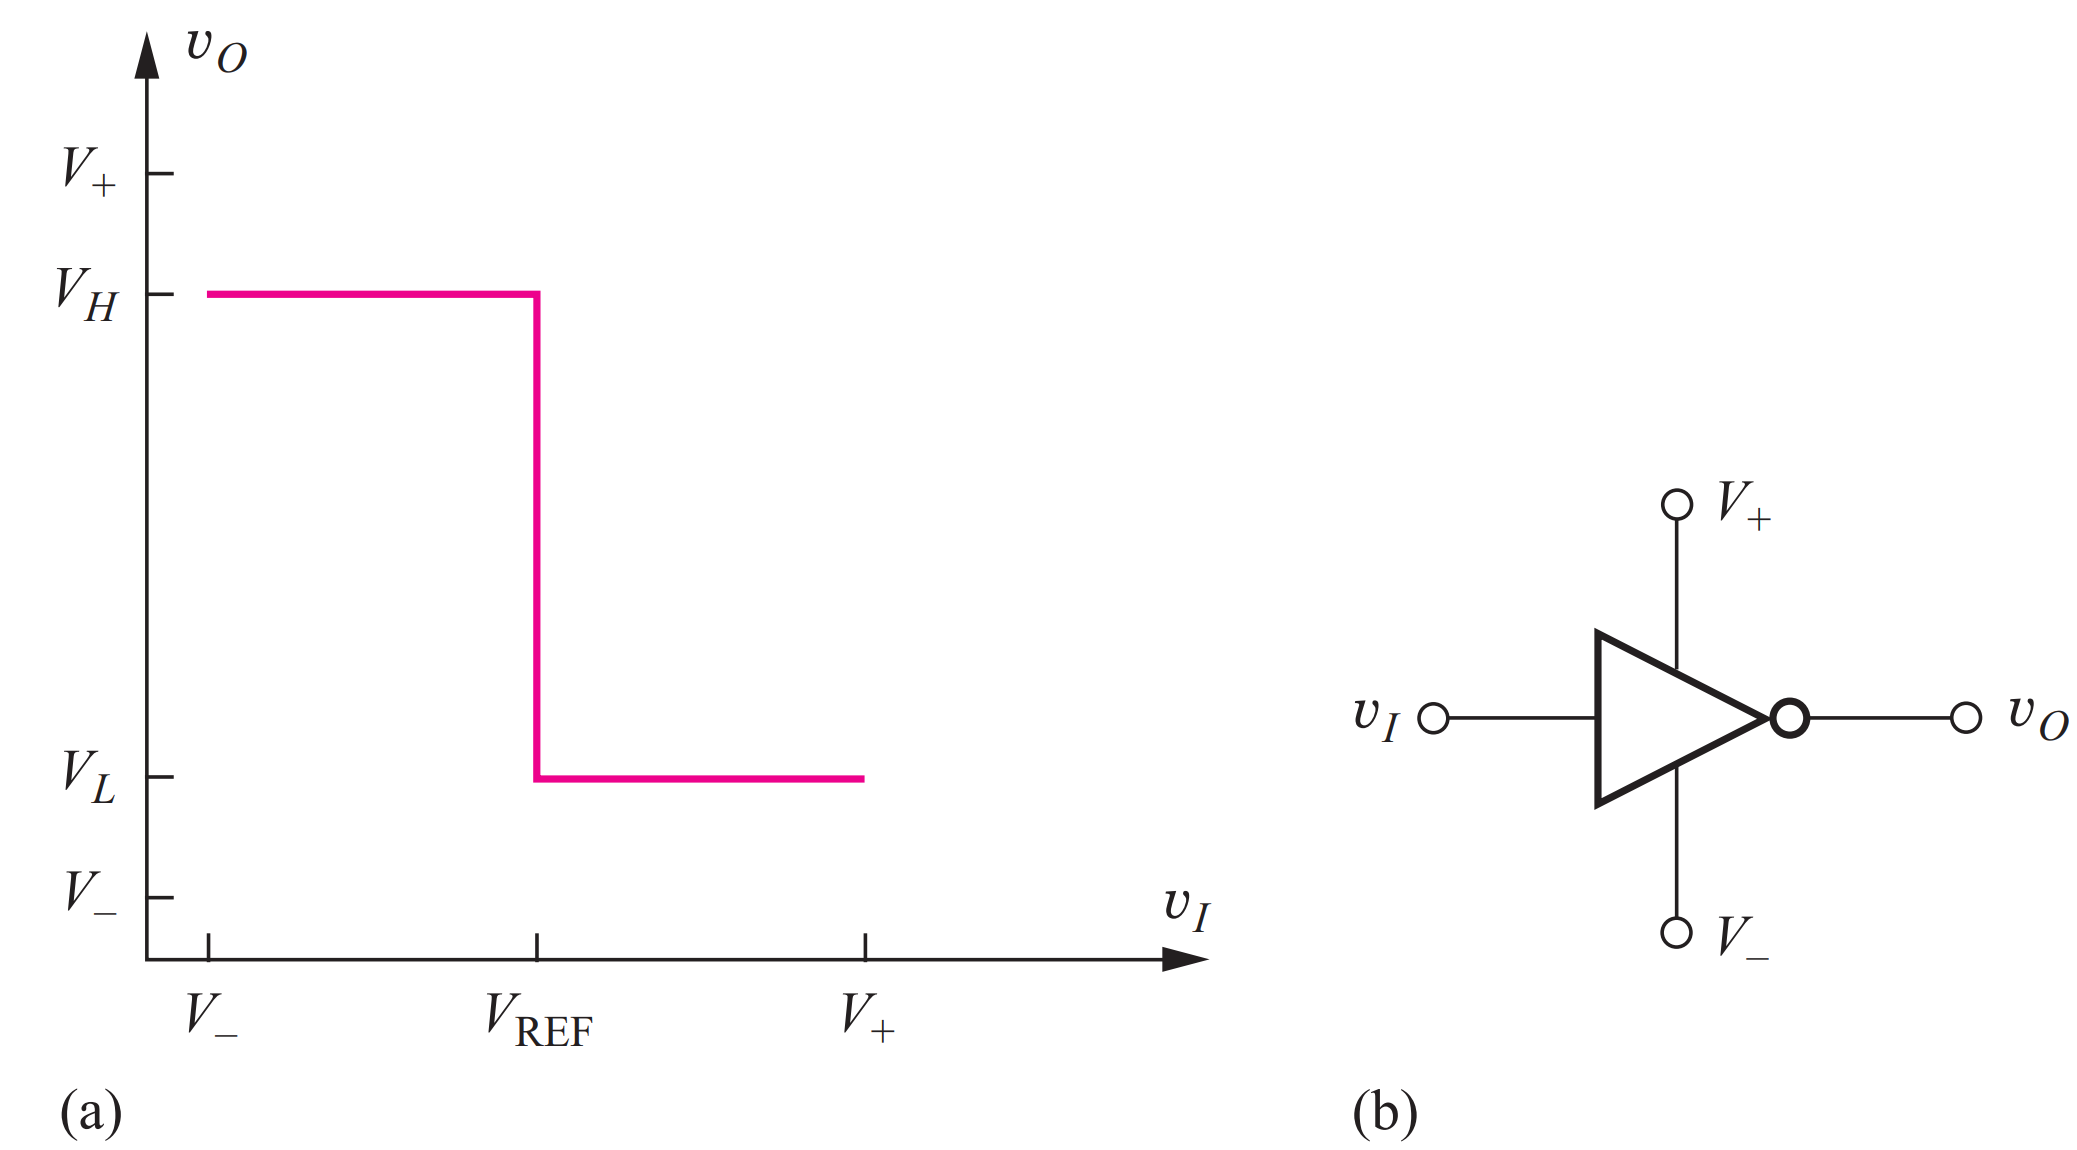
\includegraphics[width=0.75\linewidth]{img/inverter.png}
    \caption{Funzione ingresso/uscita e simbolo circuitale}    
\end{figure}

\subsection{Schema di base dell'invertitore}

Per ottenere il risultato che ci aspettiamo da un invertitore dobbiamo utilizzare due circuiti in modo tale da pilotare l'uscita verso il valore logico alto o basso, chiamati \textbf{pull-up} e \textbf{pull-down}.

\begin{itemize}
    \item[] La	rete	di	pull	down	porta	l’uscita	al	valore	basso;
    \item[] La	rete	di	pull	up	porta	l’uscita	al	valore	alto.
\end{itemize}

Dunque le tensioni in ingresso NON vengono usate per portare l'uscita al valore desiderato per solamente per attivare i due circuiti, è il circuito di pull-up/down che pilota l'uscita.

In questo modo la tensione in uscita tende verso il valore del circuito che "tira più forte".


\begin{figure}[htbp]
    \begin{minipage}[htbp]{0.5\textwidth}
    \centering
        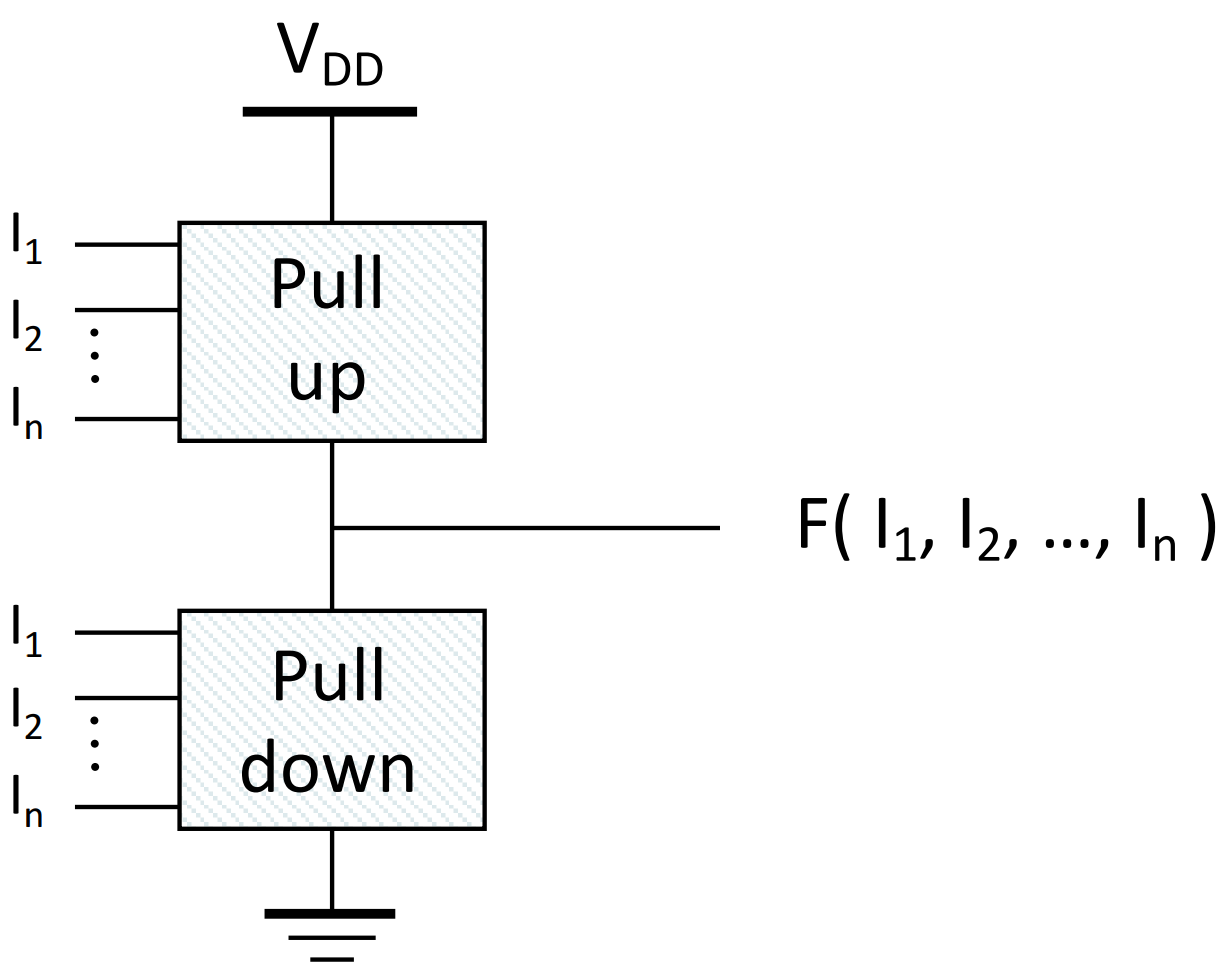
\includegraphics[width=0.6\linewidth]{img/pull_u_d.png}   
    \end{minipage}
    \begin{minipage}[htbp]{0.5\textwidth}
    \centering

    \begin{tabular}{c|c c}
             & \textbf{Pull-up OFF} & \textbf{Pull-up ON} \\
             \hline
        \textbf{Pull-down OFF} & Z (float)\footnote{alta impedenza, l'uscita può mantenere il livello, scaricarsi o caricarsi anche rispetto alle condizioni circostanti dato il fenomeno del campo magnetico generato attorno al filo} & 1 \\
        
        \textbf{Pull-down ON} & 0 & Dipende\footnote{Il circuito è come un partitore di tensione, chi tira di più vince} \\
    \end{tabular}
    
    \end{minipage}
\end{figure}


% \begin{figure}[htbp]
%     \centering
%     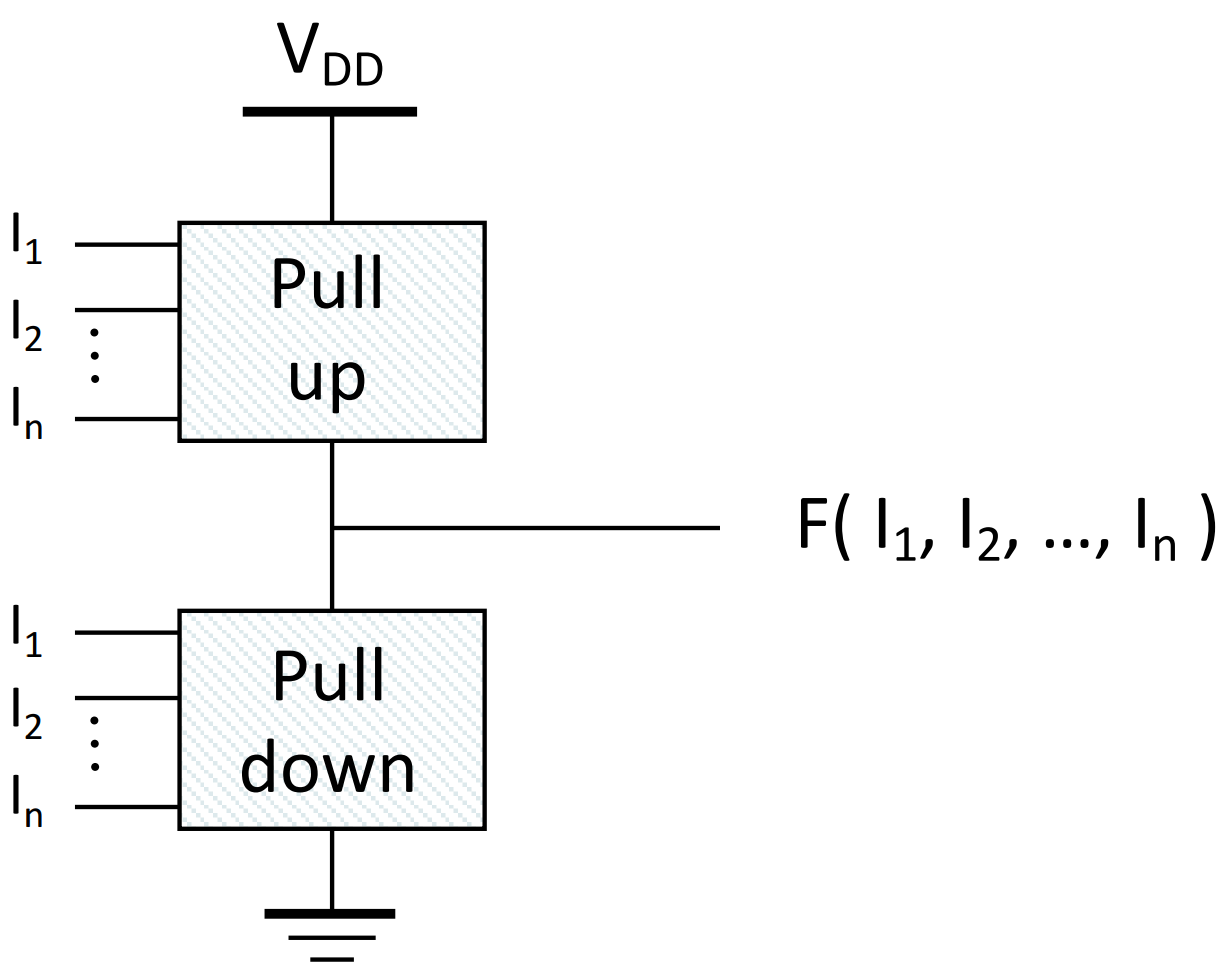
\includegraphics[width=0.35\linewidth]{img/pull_u_d.png}    
    
% \end{figure}

% \begin{table}
% \centering
%     \begin{tabular}{|c|c|c|}
%         \hline
%              & \textbf{Pull-up OFF} & \textbf{Pull-up ON} \\
%         \hline
%         \textbf{Pull-down OFF} & Z (float)\footnote{alta impedenza, l'uscita può mantenere il livello, scaricarsi o caricarsi anche rispetto alle condizioni circostanti dato il fenomeno del campo magnetico generato attrono al filo} & 1 \\
%         \hline
%         \textbf{Pull-down ON} & 0 & Dipende\footnote{Il circuito è come un partitore di tensione, chi tira di più vince} \\
%         \hline
%     \end{tabular}
% \end{table}


\subsection{Interruttore	con	carico	resistivo}

Il modo di realizzare un invertitore è quello di creare dei cammini verso $\vdd$ e verso massa. L'inverter più semplice è quello denominato a \textbf{carico resistivo} costituito da una resistenza che collega sempre l'uscita a $\vdd$ con un impedenza diversa da zero la quale tira verso l'alto; e un circuito di pull-down realizzato con un transistore 	MOS, interruttore, che quando $v_i$ è bassa, 	l’interruttore	è	aperto (non tira verso massa) e l'uscita è alta, fase di \textbf{\textit{pull-up}}.


% In questo caso tanto è più grande è la resistenza, tanto più la corrente fa fatica a passare (circuito aperto) e quindi tanto è più alta la differenza di potenziale tra \vp e \vo.

% DA RIGARDARE QUESTA ILTIMA FRASE


\paragraph{}

Quando $v_i$ è	alta,	l’interruttore	è	chiuso,	e	l’uscita	è	connessa	a	
massa	dal	transistore, se quest'ultimo tira più forte di R, a massa, fase di \textit{pull down}.

\begin{figure}[htbp]
    \centering
    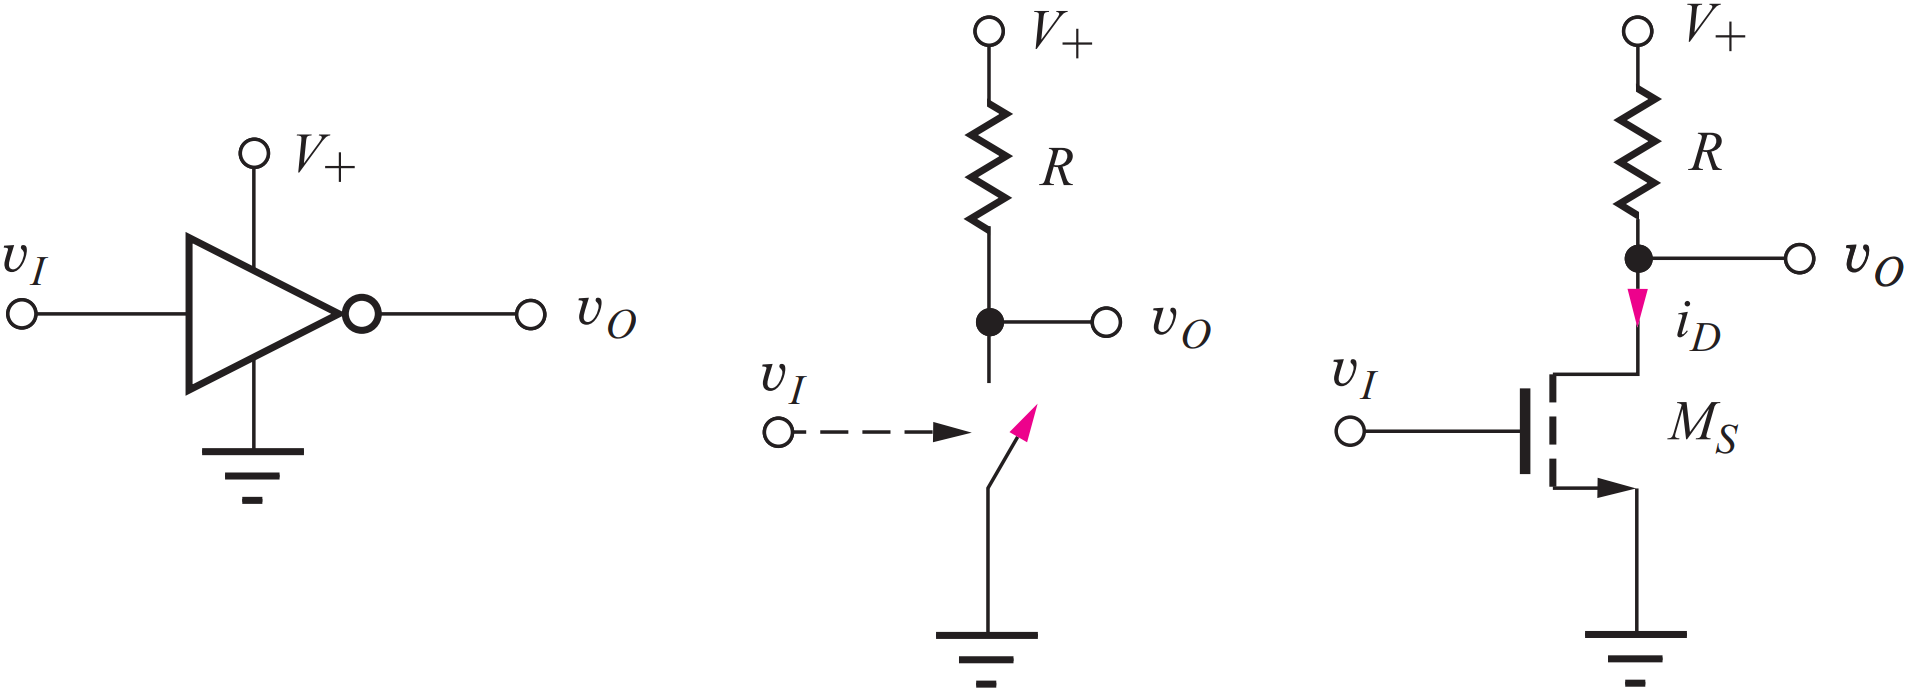
\includegraphics[width=0.55\linewidth]{img/interr_resist.png}
\end{figure}
\section{Caratteristica reale}
Ovviamente prima abbiamo visto un grafico dove si mostrava il comportamento ideale di questo circuito, in realtà l'andamento non sarà lineare. Agli estremi troveremo le zone che interessano ai circuiti elettronici digitali, i quali rappresentano 0 o 1, mentre della zona centrale è detta di \textbf{amplificazione}.

\begin{figure}[htbp]
    \centering
    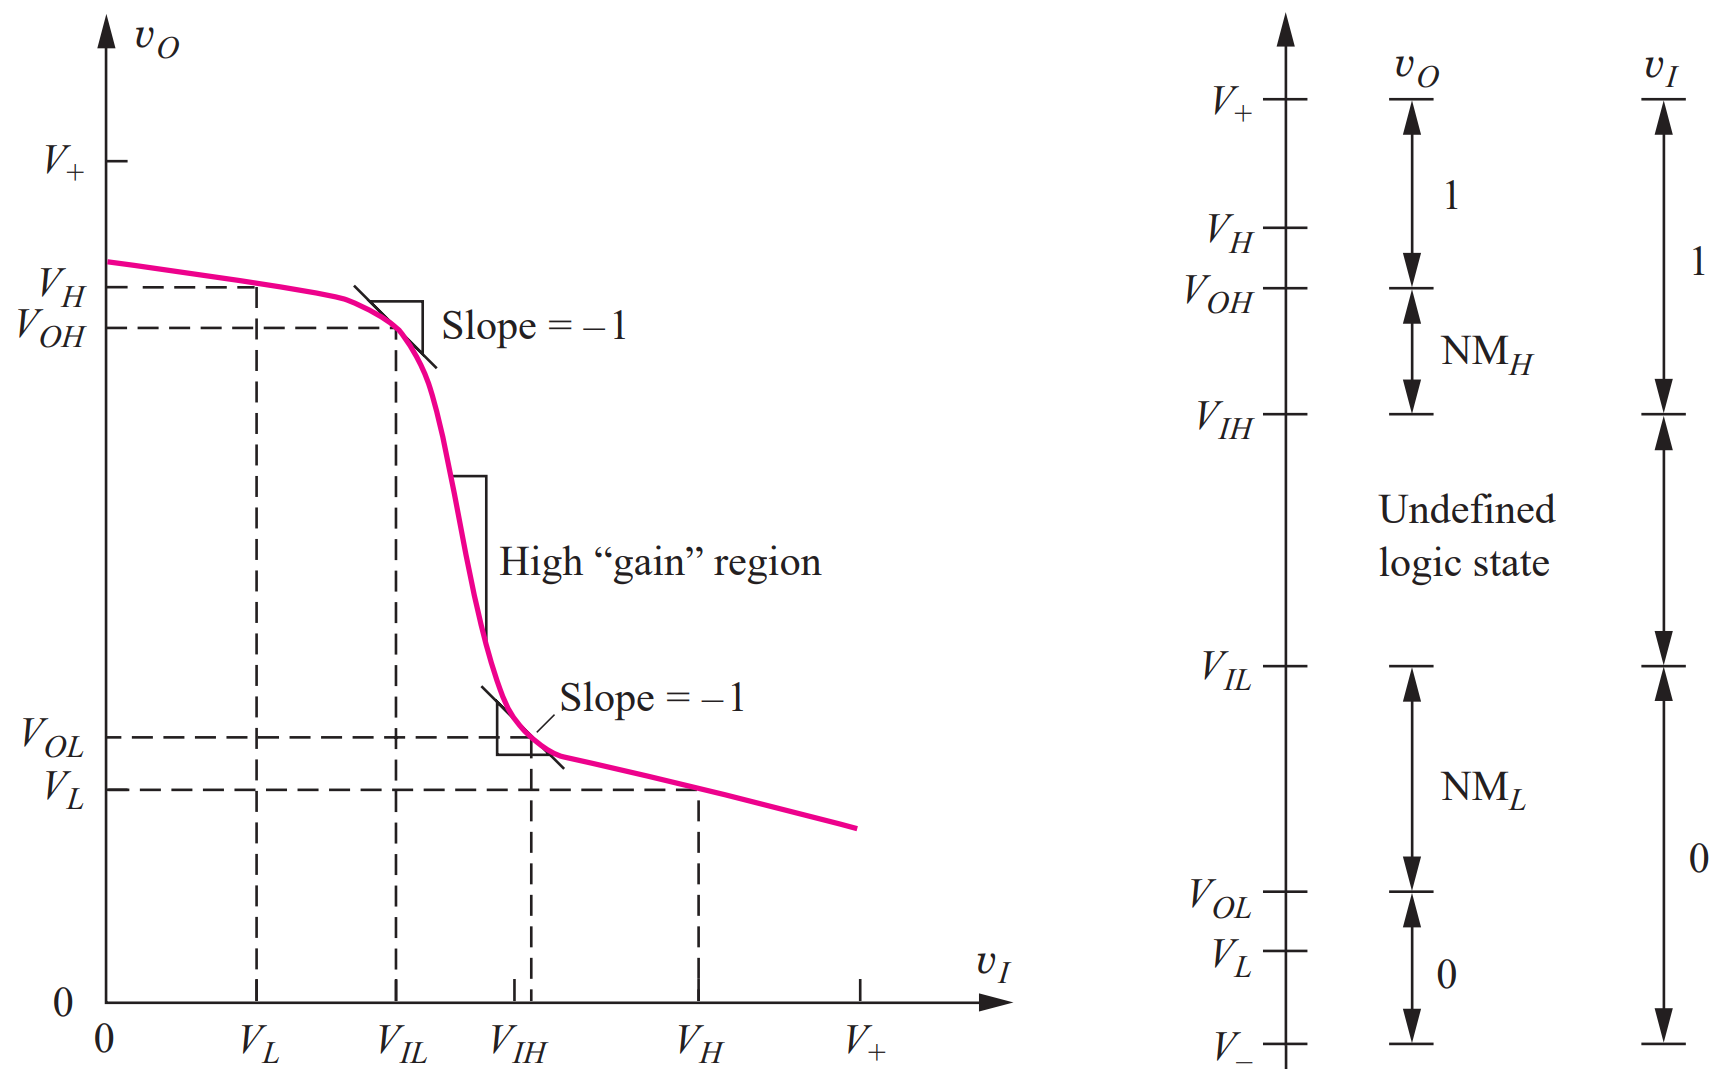
\includegraphics[width=0.75\linewidth]{img/grafico_invert_resist.png}
    \caption{Caratteristica reale invertitore resistivo}    
\end{figure}


\newpage
\section{Margini di rumore}

Come posso definire il cambiamento dello stato? Una prima grossolana approssimazione potrebbe essere quella di dividere a metà, con una soglia, la tensione di alimentazione. Tutto quello che sta al di sopra lo possiamo considerare altro e quello che sta sotto basso.

Questo metodo però non porterebbe a risultati ottimali in quanto se un segnale è a ridosso della soglia, solo un po' di rumore porterebbe a far variare l'uscita.

\paragraph{}
Dunque una soluzione è quello di stare lontano dalla soglia e avere un\textbf{ margine di errore}. Come possiamo definirlo questo margine di errore?

Osservando quando nel grafico della caratteristica si incontrano i punti in cui la tangente alla curva tende al valore $-1$: le	tensioni	per	le	quali	la	tangente	vale	$-1$ discriminano	il	livello	alto	e	basso.

Questo perché possiamo discriminare le parti del circuito che si comportano come amplificazione, infatti nella zona centrale la derivata ha un numero in valore assoluto più grande di 1, quindi presenta un amplificazione.

Le zone più esterne invece, dove la tangente ha un valore $-1 < x < 0$, l'inverter attenuerà, in particolar modo se vi è del rumore ne riduce di molto la componente.  

\paragraph{Notazione: }

\begin{itemize}
    \item[$\blacktriangleright$]    \textbf{\vil} : tensione	massima	per	la	quale l’ingresso	è	considerato	basso;

    \item[$\blacktriangleright$] \textbf{\vih} : tensione	minima	per	la	quale l’ingresso	è	considerato	alto;

    \item[$\blacktriangleright$] \textbf{\vol}: valore estremo	di	uscita	per \vi = \vih;
    \item[$\blacktriangleright$] \textbf{\voh}: valore  estremo di uscita per \vi = \vil.
    \item[$\blacktriangleright$] \textbf{\vol}: valore estremo	di	uscita	per \vi = \vih;
    \item[]
    \item[$\blacktriangleright$] $NM_H = V_{OH} - V_{IH}$ 
    \item[$\blacktriangleright$] $NM_L = V_{IL} - V_{OL}$ 
\end{itemize}

La zona di mezzo, amplificazione, per questa tipologia di scopo e circuiti non si dovrà considerare.


\paragraph{}

Utilizzando più porte logiche, se l'ingresso abbiamo \vih, in uscita ci troviamo \vol, la quale a sua volta deve essere riconoscere come tensione bassa.

Dunque $V_{OL}$ deve essere inferiore alla massima tensione che l'inverte a valle riconosce come bassa che è \vil : \vol $\,\leq\,$ \vil, se verificata il circuito funziona.

Nel caso opposto avremo che: \voh $\,\geq\,$ \vih. 

\paragraph{}
Questa differenza è definita \textbf{Margine di rumore}.


\begin{figure}[htbp]
    \centering
    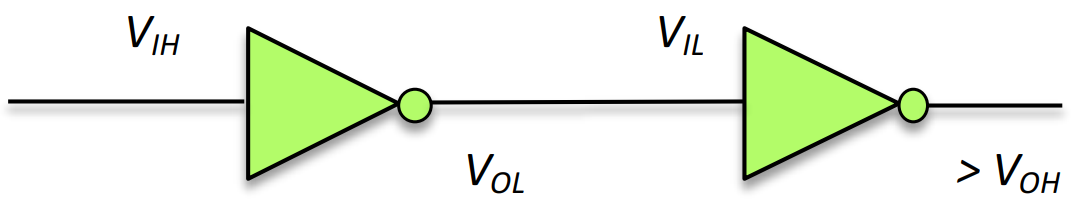
\includegraphics[width=0.45\linewidth]{img/cascata.png}    
    
\end{figure}

\newpage
\section{Obiettivi di progetto}
Ora dobbiamo progettare l'inverter in modo tale da renderlo migliore:

\begin{itemize}
    \item Minimizzare la regione indefinita, la caratteristica deve essere la più verticale possibile;
    \item Massimizzare i margini di rumore, dunque oltre al rumore nel circuito potremmo utilizzare componenti con tolleranze più grandi (processo meno preciso = costo minore);
    \item Dispositivo unidirezionale, l'uscita non deve influenzare l'ingresso; 
    \item I livello di I/O devono essere compatibili, ovvero margini di rumori positivi, se fossero negativi non potremmo costruire circuiti in casata;
    \item Massimizzare gli indici le prestazioni:
    \begin{itemize}
        \item Area più piccola possibile (costo minore);
        \item Minimizzare i consumi di potenza;
        \item Operare alla massima velocità;
    \end{itemize}
\end{itemize}

Normalmente gli indici di prestazione sono in conflitti tra di loro.

\section{Circuito invertitore nMOS}

Il circuito per realizzare un invertitore è uguale all'amplificatore utilizzato in zona non lineare.

\begin{figure}[htbp]
    \centering
    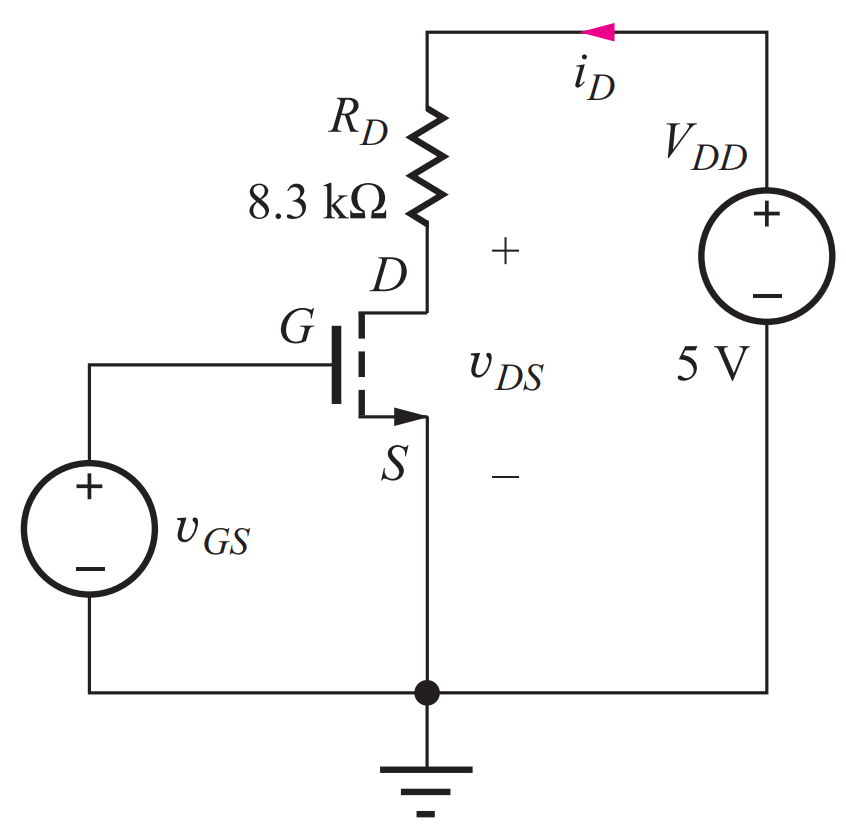
\includegraphics[width=0.35\linewidth]{img/calcolo_retta_carico.png}
    \caption{Circuito}    
\end{figure}

L'uscita la prendiamo attaccando un filo sul drain: $\vds = V_O$. A questo punto, al contrario dell'analisi, ora dobbiamo progettarlo con determinate prestazioni.

Messo per iscritto che utilizzeremo un inverter a carico resistivo e che la topologia sia quella in figura, dobbiamo scegliere: la dimensione di R e determinare il valore del rapporto $W/L$.

La L normalmente viene fissata con la tecnologia minima di produzione in quel momento (180 nm, 20 nm, ecc) si sceglie L più piccola in modo da portare più corrente possibile e minore dunque sarà la W e in generale il transistore diventa più piccolo.

\subsubsection{Obiettivo:}

\begin{itemize}
    \item[--] Rendere \vl $\,$ abbastanza bassa (sicuramente più bassa della $\vgs$) e \vh $\,$ = $\vdd$;
    \item[--] Minimizzare il consumo di potenza;
    \item [--] Massimizzare le prestazioni
\end{itemize}

\subsection{Scelta di \vl}

\textbf{La	tensione	di	uscita:}	deve	pilotare	la porta	logica	successiva, ovvero deve mettere in interdizione il gate del transistor successivo per metterlo in cut-off: \vl < $\vtn$, solitamente un valore appropriato si aggira tra 25\% e il 50\% di $\vtn$.

Nei transistori normalmente la $\vtn = 0.6V$, dunque possiamo scegliere una \vl $= 0.2V$, ovvero un terzo.
\paragraph{}
\textbf{Consumi di potenza:} Se il transistore è interdetto il generatore non eroga corrente (a meno quella per caricare il gate del transistor a valle), anche se la tensione rimane alta.

Quando \vi $\,$ è alta, scorre corrente e si consuma la batteria. Supponendo $\vdd = 2.5V$, vicino agli standard di oggi, scegliendo un consumo di potenza che ci aggrada, P = 0.2 mW, dettato dai parametri come: 

\begin{itemize}
    \item energia disponibile nella batteria;
    \item numero di porte logiche;
    \item la media di quante queste hanno l'uscita a zero;
    \item quanta potenza il sistema riesce a dissipare.
\end{itemize}

Partendo dal consumo totale ad esempio 0.2 W perché così so che la batteria mi dura due giorni, calcolando 2000 porte logiche di cui la metà a valore logico altro (potenza = 0), ottengo che ogni porta logica dovrà consumare 0.2 mW.


\subsection{Dimensionamento}
Come detto precedentemente supponiamo:
\begin{equation*}
    \vtn = 0.6V \qquad\qquad \vdd = 2.5V \qquad\qquad K_n' = 100\mu A/V^2
\end{equation*}

Per soddisfare i consumi di potenza:

\begin{equation*}
    \vdd \cdot I_D = 0.2 mW \qquad \longrightarrow \qquad I_D = 0.2 / 2.5 = 80 \mu A
\end{equation*}
Questa è la corrente che deve scorrere quando l'uscita è bassa (la porta consuma).

\paragraph{Calcolo R:}

\begin{equation*}
    I_D \cdot R = 2.5 - V_L = 2.5 - 0.2 \qquad \longrightarrow \qquad R = (2.5 - 0.2 ) / 0.00008 = 28.75 K\Omega
\end{equation*}
Si poteva anche ottenere grazie alla retta di carico, supponendo di avere un transistore discreto.

\paragraph{Calcolo il rapporto di forma W/L:}

\begin{equation*}
    V_i = \vgs = V_h = 2.5 V \text{,  } \qquad \vds = 0.2V
\end{equation*}

Trovandoci in zona triodo ($\vgs\,$ molto alta, $\vds\,$piccola, la tensione di soglia è 0.6 V, quindi $0.2 + 0.6 = 0.8V$ la $\vgs$ è molto più alta e dunque siamo in zona triodo) possiamo utilizzare la formula della zona triodo per trovare il rapporto W/L:

\begin{equation*}
    \frac{W}{L} = \frac{80 \mu A}{100 \frac{\mu A}{V^2} (2.5-0.6-\frac{0.2}{2})0.2} = 2.22 = \frac{2.22}{1}
\end{equation*}

Ora abbiamo tutti le dimensioni dei componenti. 

Non abbiamo considerato in questo caso le tempistiche. Queste ultime dipendono da quanto veloce la resistenza riesca a caricare il/i condensatore/i (gate) a valle.

Più piccola sarà R  più passa corrente e più verrà caricato in fretta il gate, per calcolare il tempo dobbiamo considerare il circuito come se fosse un RC, e con $\tau = RC$ ci possiamo ricavare quanto tempo impiega a caricarsi e scaricarsi.
\paragraph{}
Scegliendo una R piccola però significa che, si andremo più veloci, ma stiamo consumando anche più corrente. Vi è sempre lo scontro prestazioni e consumi.


\subsection{Calcoliamo i margini di rumore: \vil $\,$ e \voh}
Quando \vi $\,$ = $\vgs$ è piccola, ma maggiore della tensione di soglia, e \vo $\,$ = $\vds$ è grande ci troviamo sicuramente in \textbf{saturazione}.

Utilizzando la corrente di drain e il valore dell'uscita \vo = $\vdd - I_DR$, otteniamo:

\begin{equation*}
    V_o = V_{DD} - \frac{K_n}{2}(V_{GS}-V_{TN})^2 R
\end{equation*}

Cerchiamo dunque quando la tangente vale $-1$: la si ottiene facendo il rapporto tra la derivata in uscita e la derivata in ingresso

\begin{equation*}
    \frac{dV_o}{dV_{GS}} = - K_n(V_{GS}-V_{TN})R = -1
\end{equation*}

\begin{equation*}
    V_{IL} = V_{GS} = V_{TN} + \frac{1}{K_nR}
\end{equation*}

\begin{equation*}
    V_{OH} = V_{DD} - \frac{1}{2K_nR}
\end{equation*}


\begin{figure}[htbp]
    \centering
    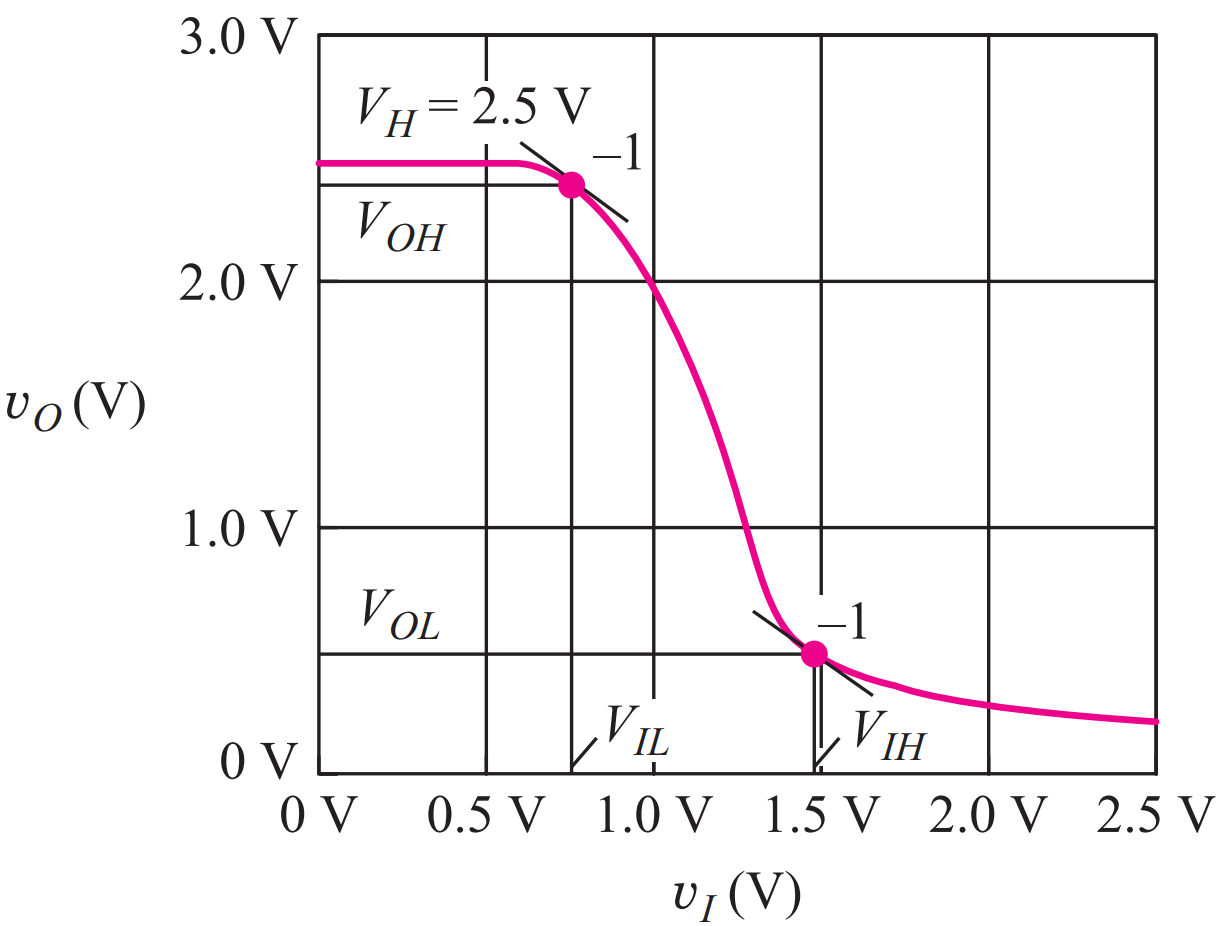
\includegraphics[width=0.5\linewidth]{img/plot_.png}
    
    
\end{figure}

Per il valore logico alto, quando \vi $\,$= $\vgs$ è grande \vo $\,$= $\vds$ è piccola siamo in zona triodo. Come prima dobbiamo sempre derivare e uguagliare a -1, in questo caso la derivata risulterà più complicata, infatti risulta più semplice assumere che: $\frac{dV_o}{dV_{GS}} = \frac{dV_{GS}}{dV_o}^{-1}$

Il risultato diverrà:

\begin{equation*}
    V_O= \vdd - K_n\Biggl(\vgs- \vtn - \frac{V_O}{2}\Biggl)V_O R
\end{equation*}

\begin{equation*}
    K_nR\vgs - K_nR\vtn - \frac{K_nR}{2}V_O - \frac{\vdd}{V_O} = -1
\end{equation*}


\begin{equation*}
    K_nR\vgs = -1 + K_nR\vtn - \frac{K_nR}{2}V_O + \frac{\vdd}{V_O}
\end{equation*}


\begin{equation*}
    \vgs = -\frac{1}{K_nR} + \vtn + \frac{1}{2}V_O + \frac{1}{K_nR}\frac{\vdd}{V_O}
\end{equation*}

\begin{equation*}
    \frac{d\vgs}{dV_O} = \frac{1}{2} -  \frac{1}{K_nR}\vdd \frac{1}{V_O^2} = -1
\end{equation*}

\begin{equation*}
    \frac{3}{2}V_O^2 = \frac{\vdd}{K_nR} \qquad \longrightarrow \qquad V_O = \Bigg(\frac{2}{3}\frac{\vdd}{K_nR}\Bigg)^{\frac{1}{2}}
\end{equation*}

\begin{equation*}
    \vgs = \vt - \frac{1}{K_nR} + \frac{1}{2}\Bigg(\frac{2}{3}\frac{\vdd}{K_nR}\Bigg)^{\frac{1}{2}} + \frac{\vdd}{K_nR}\Bigg(\frac{3}{2}\frac{K_nR}{\vdd}\Bigg)^{\frac{1}{2}} = \vt - \frac{1}{K_nR} + \frac{1}{2}\Bigg(\frac{2}{3}\frac{\vdd}{K_nR}\Bigg)^{\frac{1}{2}} + \Bigg(\frac{3}{2}\frac{K_nR}{\vdd}\Bigg)^{\frac{1}{2}}
\end{equation*}

Pertanto:

\begin{equation*}
   V_{IH} = \vtn - \frac{1}{K_nR} + 1.63\Bigg(\frac{\vdd}{K_nR}\Bigg)^{\frac{1}{2}}
\end{equation*}

\begin{equation*}
    V_{OL} = \sqrt{\frac{2\vdd}{3K_nR}}
\end{equation*}

\paragraph{Esempio di calcolo}

Per il nostro invertitore abbiamo deciso i seguenti valori: $\vtn = 0.6V$, $K_n = 100\cdot2.22 = 222\,\mu A/V^2$, $R = 28.8\,K\Omega$,  $K-nR = 6.39$, sostituendo i valori otteniamo i seguenti valori:

\begin{itemize}
    \item $V_{IL} = 0.756 V$ il massimo valore che viene riconosciuto come basso dall'inverter;
    \item $V_{IH} = 1.46 V$ ingresso minimo che viene riconosciuto come alto;
    \item $V_{OH} = 2.42 V$ uscita in corrispondenza di $V_{IL}$, vicina a 2.5V;
    \item $V_{OL} = 0.51 V$ uscita in corrispondenza di $V_{IH}$, vicina a 0.5V comunque sotto la soglia anche se di poco.
\end{itemize}

Calcolo dei margini di rumore:

\begin{equation*}
    NM_H = V_{OH} - V_{IH} = 0.96V \text{ è un buon valore: si ha quasi un volt di tolleranza}
\end{equation*}
\begin{equation*}
    NM_L = V_{IL} - V_{OL} = 0.25 V \text{ non un buon valore: si ha poco margine}
\end{equation*}

\subsubsection{Resistore}

Dobbiamo preoccuparci anche di come costruire il resistore sul circuito integrato. La resistenza sappiamo che dipende dalla resistività:

\begin{equation*}
    R = \rho \frac{L}{TW} = 28.8\,K\Omega
\end{equation*}

Vogliamo T e W piccole e la lunghezza L lunga per avere una resistenza elevata. Supponiamo che $T = 1\,\mu m$, $\rho = 0.001 \,\Omega cm$, e con una tecnologia produttiva di un micron mettiamo $W = 1\,\mu m$. Facendo così però la lunghezza dovrà essere: $2880\,\mu m$, una cosa gigantesca se si pensa che un circuito integrato abbastanza grande è $2\times2 \,cm$.

Ma soprattutto è enorme rispetto al solo transistor ($W/L = 22.2$, con $L=1\,\mu m$) il quale avrà un area di $2.22\, \mu m^2$ a confronto con i $2880\, \mu m^2$ della resistenza.

Dunque le resistenza nei circuiti integrati sono di difficile realizzazione anche per il fatto che il silicio non è un materiale adatto all'isolamento elettrico.
\paragraph{}

Per ovviare a questo problema cerchiamo di 	realizzare	il	carico	con	un	altro	transistore in particolare un altro nMOS con gate a potenziale fisso.

\begin{figure}[htbp]
    \centering
    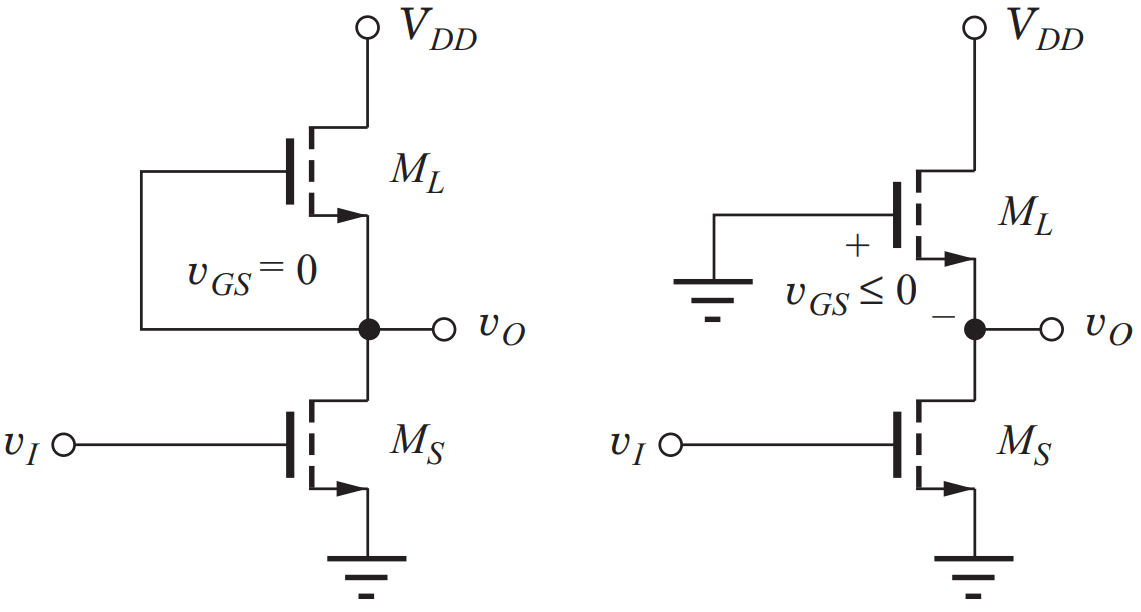
\includegraphics[width=0.5\linewidth]{img/nMOS_fisso.png}    
    
\end{figure}

I due circuiti sopra in figura non funzionano quando:

\begin{itemize}
    \item Nel primo caso, $V_{GS} = 0$, quindi $M_L$ è	sempre	interdetto
    \item Nel secondo caso, $V_{GS} < 0$, quindi $M_L$ è	sempre	interdetto
\end{itemize}

Una topologia che potrebbe funzionare potrebbe essere la seguente

\newpage
\section{Inverter con carico saturato}

    \begin{figure}[htbp]
        \centering
        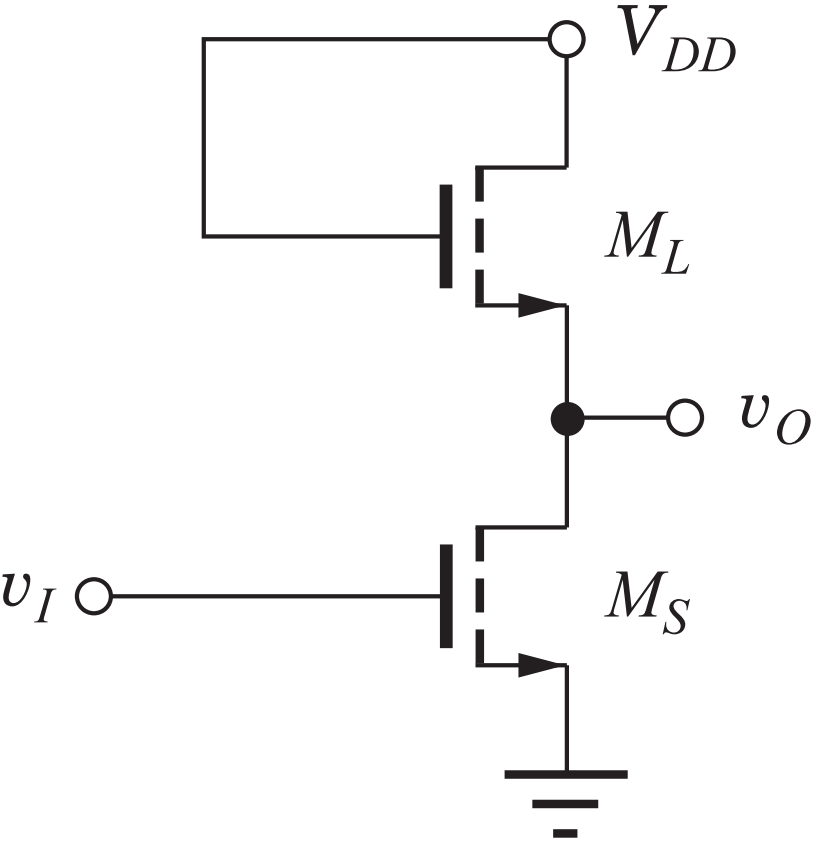
\includegraphics[width=0.25\linewidth]{img/Inverte_saturato.png}        
        
    \end{figure}

Questo transistore, $M_L$, si potrà trovare o in zona di cut-off o in zona di saturazione, quasi sempre sarà in quest'ultima. Questo tipo di carico viene chiamato saturato perché appunto il transistore sarà in saturazione.
\paragraph{}

Il problema di questo circuito è che il source di $M_L$ è collegato all'uscita e quest'ultima quando è bassa rimane tale, ma quando è alta vogliamo un uscita alta ma il source rischia di non essere così alto, inoltre se vi è una differenza di tensione tra source e substrato che comporta ad avere un effetto body che \textbf{modifica la tensione di soglia} ($V_{SBL} = V_O$), e in questo caso non potremmo trascurarlo quando l'uscita dovrà andare a valore alto.

\paragraph{}
Utilizziamo gli stessi parametri a carico resistivo:

\begin{itemize}
    \item $I_D = 80 \mu A$
    \item $V_{DD} = 2.5 V$
    \item $V_L = 0.2 V$ tensione che deve assumere l'uscita quando si vuole in output un valore logico basso
    \item $I_D$, formula per la zona si saturazione
    \item $V_{GSL} =V_{DD} - V_O$
    \item $\gamma = 0.5 $
    \item $2\phi_f = 0.6$
\end{itemize}

\subsection{Dimensionamento}

\begin{equation*}
    V_{TNL} = V_{T0} + \gamma(\sqrt{V_{SB} + 2\phi_F}  - \sqrt{2\phi_F}) = 0.6 + 0.5(\sqrt{0.2+0.6} - \sqrt{0.6}) = 0.66V
\end{equation*}

Imponendo la corrente di drain troviamo il rapporto di forma:

\begin{equation*}
    \frac{W}{L} = \frac{2I_D}{K_n'(V_{GS}  - V_{TNL})^2} = \frac{2\cdot80 \mu A}{100 \frac{\mu A}{V^2}(2.3-0.66)^2} = \frac{1}{1.68}
\end{equation*}

Otteniamo dunque che la dimensione del carico è addirittura più piccola, $1.68 \,\mu m^2$, che è simile a quella del driver, ma è più grande della tecnologia utilizzata ($1 \,\mu m$) perché non vogliamo che il circuito resistivo porti troppa corrente (ne porta circa un quarto rispetto al pull-down), infatti vogliamo che il pull-down vinca quando deve tirare giù, e dunque il pull-up deve essere più debole (sempre per il partitore di tensione).

\begin{figure}[htbp]
    \centering
    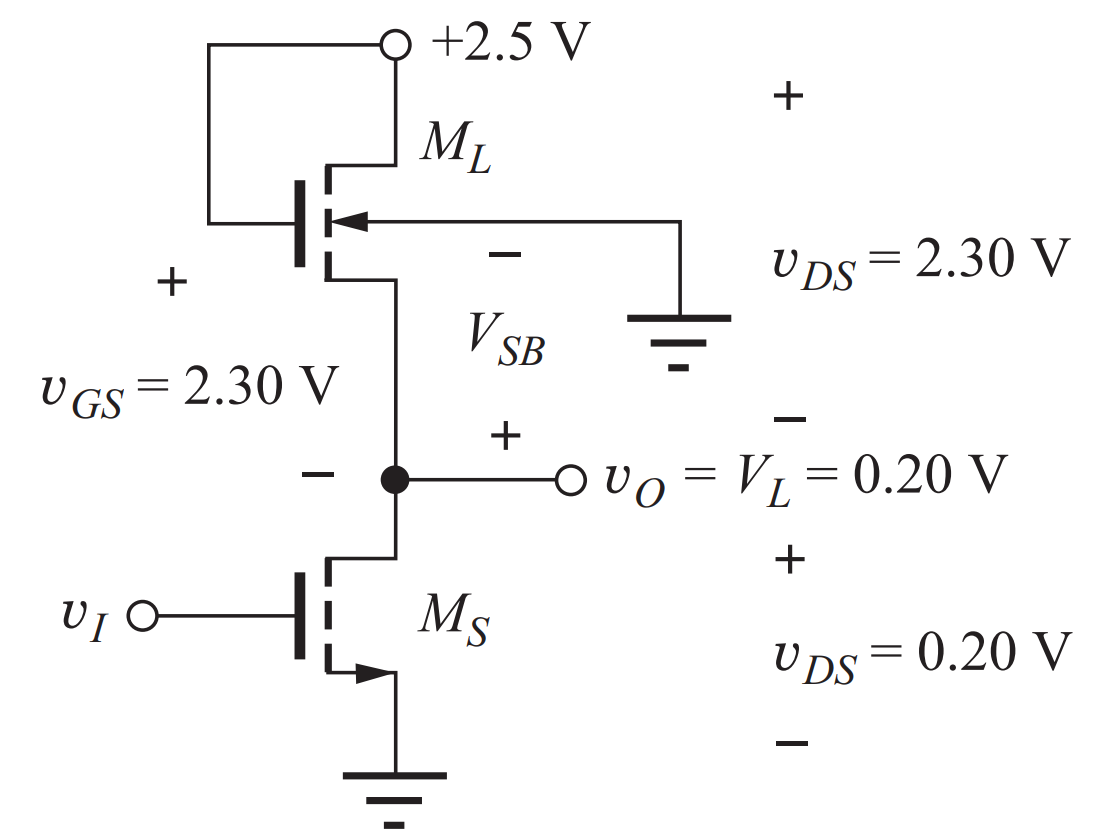
\includegraphics[width=0.4\linewidth]{img/pull_uppp.png}    
    
\end{figure}

\newpage
\subsection{Calcolo di $V_H$}
Ovviamente anche in questo caso vi sono degli svantaggi. Infatti quando l'ingresso è basso, $V_I =V_L$ , il pull-down si interdice è l'uscita dovrebbe andare a livello logico ad 1.

Il problema è che il condensatore messo a valle mentre si carica, la $V_{GSL} = V_{DD} - V_{S} \text{ (inizialmente a 0.2 V)}$, la tensione sul source aumenta fino al punto da portare la $V_{GSL}$ alla tensione di soglia, spegnendo di fatto il transistore e portando il condensatore ad un massimo di $V_O = V_{DD} - V_{GS} = 2.5 - 0.6 = 1.9V$.
\paragraph{}
In realtà non è così semplice perché man mano che $V_O$ sale e più l'effetto body ha una sua rilevanza, dunque l'uscita arriva ad un punto dell'uscita tale per cui la $V_{GS} = V_{TN}$ ma quest'ultima cambia e dunque l'uscita arriverà a $V_{DD} - V_{TNL}$ e la tensione di soglia dobbiamo calcolarla tramite l'effetto body:

\begin{equation*}
    V_O = V_{DD} - V_{TNL} = V_{DD} - \Big[V_{TO} + \gamma(\sqrt{V_O + 2\phi_F} - \sqrt{2\phi_F})\Big]
\end{equation*}

\begin{equation*}
    V_O = 2.5 - \Big[0.6 + 0.5(\sqrt{V_O + 0.6} - \sqrt{0.6})\Big]
\end{equation*}

\begin{equation*}
    V_O = 1.55 \text{ o } 3.27 V \text{, quest'ultima non possibile, la tensione massima è 2.5 V}
\end{equation*}

Dunque l'uscita al posto di arrivare a $2.5\,V$, arriverà a solamente $ 1.55\,V$, questo è un problema nell'utilizzo del carico saturato. Il transistore messo a valle dunque si verrà arrivare una tensione più bassa, dunque dovremmo ridimensionare pure quello.

Inoltre vengono peggiorati pure i margini di rumore.


\subsubsection{Dimensionamento $M_S$}

Dopo lo svolgimento di tutti i conti visti in precedenza con una tensione in ingresso di $1.55\,V$ al posto dei $ 2.5\,V$ troviamo che il transistore sotto deve avere un rapporto $\frac{w}{L} = \frac{4.71}{1}$.

Diminuendo l'ingresso, il pull-down deve sempre tirare $80 \,\mu A$, e per riuscirci avendo una tensione più bassa basta aumentare il transistor. Dobbiamo infatti farlo più del doppio più grosso.

\subsection{Margini di rumore: }

\begin{itemize}
    \item[] $NM_H = 1.55 - 1.12 = 0.43 \,V$, si è dimezzato
    \item[] $NM_L = 0.6 - 0.38 = 0.22 \,V$
\end{itemize}

In compenso abbiamo un circuito molto piccolo.

\begin{figure}[htbp]
    \centering
    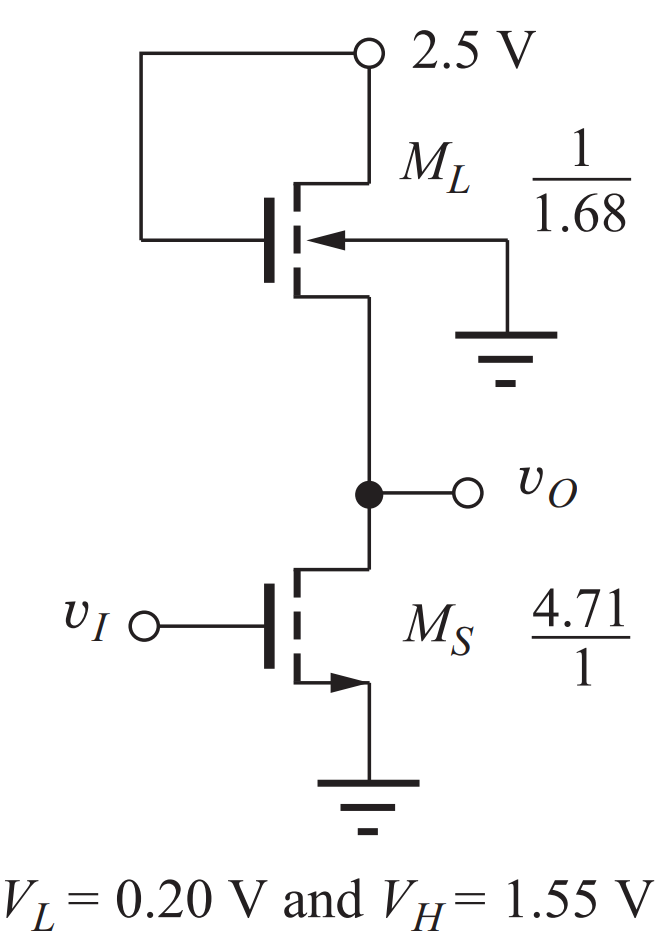
\includegraphics[width=0.25\linewidth]{img/dim_M_s.png}  
    
\end{figure}


\newpage
\paragraph{Complicanze:} il problema di questo inverter è che il pull-up si spegne perché ha una tensione di soglia troppo alta e il suo gate dopo un certo punto scende sotto questa soglia. Si potrebbe mettere allora un transistore che abbia una tensione di soglia più piccola, addirittura negativa: \textbf{carico depletion mode} o \textbf{transistore a svuotamento}.

\newpage
\section{Carico a depletion mode}

In questo caso l'ingresso $V_{GSL}$ lo collego all'uscita $V_O$, per questo il pull-up sarà sempre in conduzione, qualunque sia l'uscita, come la resistenza.

\begin{figure}[htbp]
    \centering
    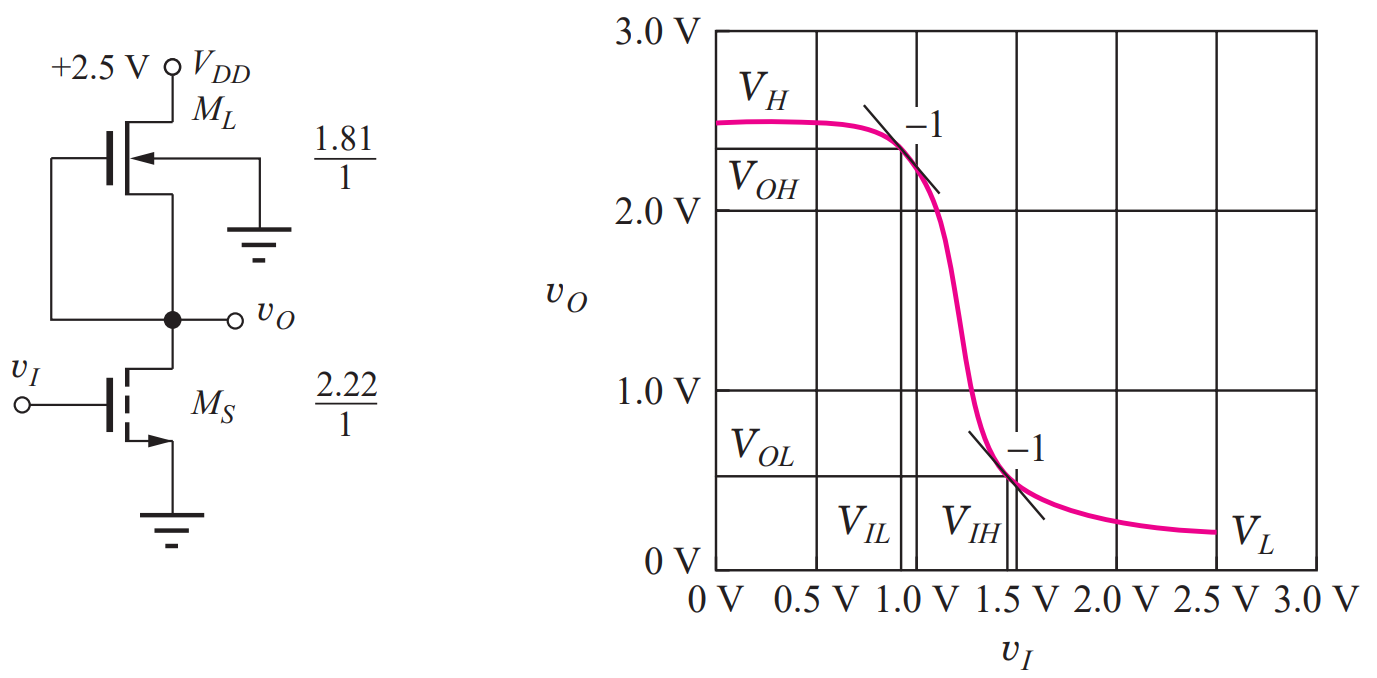
\includegraphics[width=0.75\linewidth]{img/depletion.png}
    \caption{Pull-up con transistore nMOS a svuotamento}    
\end{figure}

Vi è sempre un leggero effetto body ma è inferiore a prima.

\paragraph{}
Essendo a svuotamento, richiede un passo in più per la produzione, quindi potrebbe costare leggermente di più.

\subsection{Dimensionamento}

Usando i soliti valori e supponendo una tensione di soglia di $V_{TO} = -1 V$, anche qui è presente l'effetto body: supponiamo l'uscita bassa vediamo dove finisce la tensione di soglia.

\begin{equation*}
    V_{TNL} = V_{T0} + \gamma(\sqrt{V_{SB} + 2\phi_F}  - \sqrt{2\phi_F}) = -1 + 0.5(\sqrt{0.2+0.6} - \sqrt{0.6}) = -0.94 \,V
\end{equation*}


Ci troviamo in saturazione: $V_{DS} = 2.3 > V_{GS} - V_{TN} = 0 - (-0.94) = 0.94$ e dunque possiamo dimensionare il pull-up utilizzando la formula della saturazione

\begin{equation*}
    \frac{W}{L} = \frac{I_D}{\frac{K_n'}{2}(V_{TN}^2)} = \frac{80}{50\cdot 0.94^2} = \frac{1.81}{1}
\end{equation*}

 L'uscita in questo caso ci va a $V_{DD}$ dunque il pull-down lo dimensioniamo in egual modo se ci fosse una resistenza.


\begin{figure}[htbp]
    \centering
    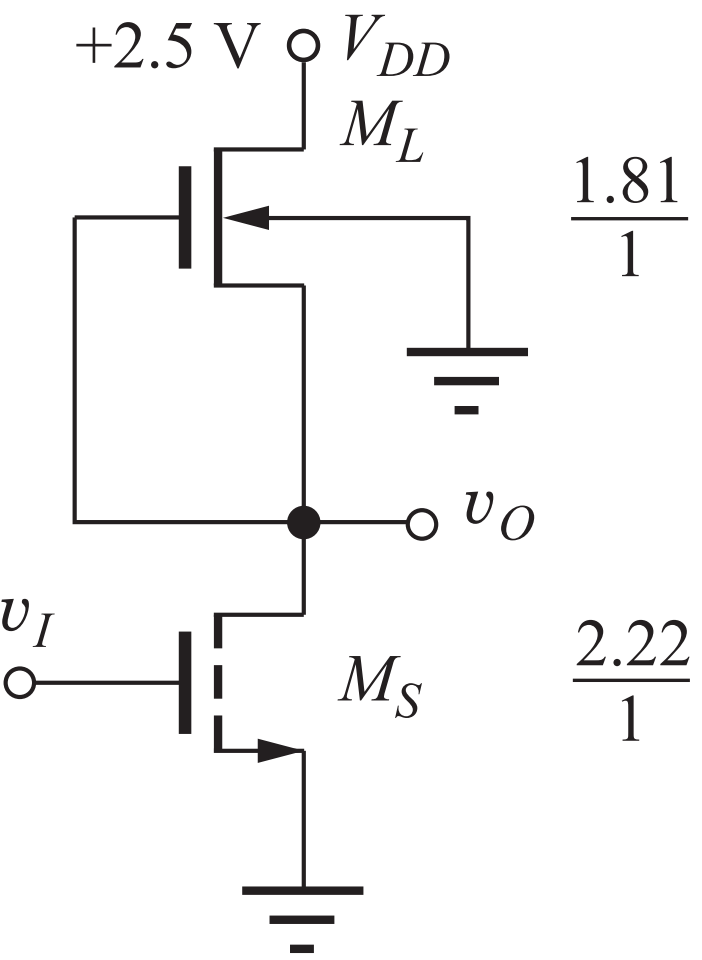
\includegraphics[width=0.25\linewidth]{img/dep_asdfv.png}    
    
\end{figure}


\newpage
\subsection{Margini di rumore: }

\begin{itemize}
    \item[] $NM_H = 2.35 - 1.45 = 0.90 \,V$, si è dimezzato
    \item[] $NM_L = 0.93 - 0.50 = 0.43 \,V$
\end{itemize}


Questo è un inverter con caratteristiche migliori a quello con carico resistivo, su molti aspetti: dimensione e margini di rumore.

\paragraph{}
Se collegassimo il gate del pull-up a $V_{DD}$? Tutto funziona ma il pull-up sarà molto forte il che vuol dire che il pull-down deve essere più forte (dimensione più grande per portare più corrente) oppure dobbiamo ridurre la potenza del pull-up facendolo molto lungo per compensare il fatto che porta tutta quella corrente.


\newpage
\section{Inverter pseudo nMOS}

Un ultima soluzione potrebbe essere quella di realizzare il pull-up tramite un pMOS. In questo caso il source è il terminale a tensione più alta il quale sarà attaccato a $V_{DD}$, il suo substrato lo attacchiamo a $V_{DD}$.

\begin{figure}[htbp]
    \centering
    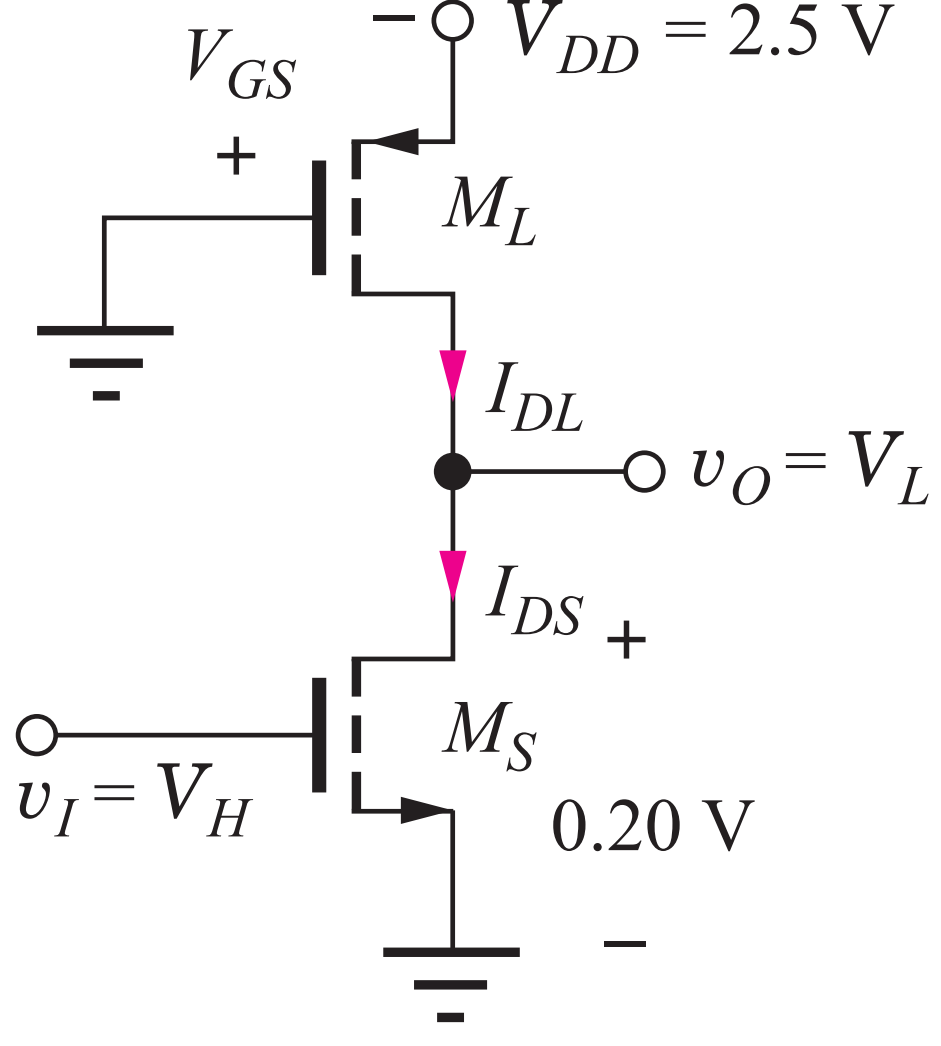
\includegraphics[width=0.27\linewidth]{img/inverter_pmos_pseudo.png}
    \caption{Inverter con carico un transistore pMOS}    
\end{figure}

\subsection{Dimensionamento}
\subsubsection{pMOS per uscita bassa:} $V_{GS} = -V_{DD} = -2.5V $; $V_{DS} = 0.2 - 2.5 = -2.3 V$; $ V_L = 0.2 V$; $V_{TP} = -0.6$. Il transistore è sempre attivo. Quando l'uscita è bassa il pMOS sarà in zona di saturazione perché $V_{GS}$ non supera $V_{DS}$ per più di una tensione di soglia $V_{TP} = -0.6 V$.

Calcoliamo dunque il rapporto di forma del transistore.

\begin{equation*}
    I_D = \frac{K_p'}{2}\frac{W}{L}(\vgs - V_{TP})^2
\end{equation*}
\begin{equation*}
    80 \mu A = \frac{1}{2}40 \frac{\mu A}{V^2}\frac{W}{L}(-2.5 + 0.6)^2
\end{equation*}
\begin{equation*}
    \frac{W}{L} = \frac{1.11}{1}
\end{equation*}

Di nuovo viene un transistore molto piccolo, o comunque simile al pull-down. 

\paragraph{}
Questo oggetto qui ci permette di far andare l'uscita fino a $V_{DD}$, quando l'uscita è alta il circuito non consuma dato che la $V_{DS} = V_{DD}$. 


\subsubsection{Uscita alta:}

Rifacendo i conti come prima viene esattamente un rapporto $\frac{W}{L} = \frac{2.22}{1}$ come con il carico resistivo.

\begin{figure}[htbp]
    \centering
    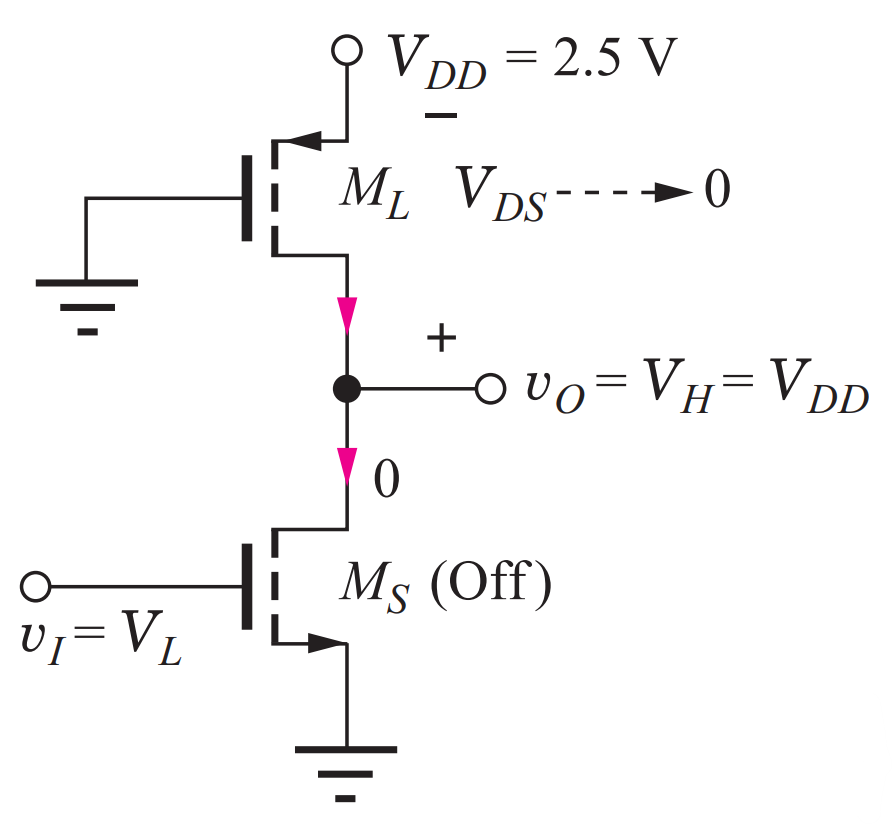
\includegraphics[width=0.37\linewidth]{img/OUTTTSS.png}    
    
\end{figure}

\subsection{Margini di rumore}
Basta	eguagliare	la	corrente	dell'nMOS con
quella	del	pMOS, differenziare $V_O$ rispetto a $V_I$ e	quindi	trovare	il	punto	in	cui	vale	$-1$, Molto	tedioso

\begin{itemize}
    \centering
    \item[] $NM_H = 2.33-1.58 = 0.75\, V$
    \item[] $NM_L = 0.95 - 0.49 = 0.46\, V$
\end{itemize}

I	margini	di	rumore	sono molto buoni. 

\paragraph{}

Tra il carico a svuotamento  e il carico a pMOS le due cose si equivalgono, magari l'altro aveva un margine del rumore $NM_H$ migliore. Anche per il pMOS vi sono dei passi in più da fare in fase di produzione dato il  substrato di tipo n.

\newpage
\section{Confronto di inverter}

\subsection{A carico resistivo}


\begin{equation*}
    I_D = \frac{V_R}{R} = \frac{V_{DD} - V_{DS}}{R} = -\frac{1}{R}V_{DS} + \frac{V_{DD}}{R}
\end{equation*}

\begin{figure}[htbp]
    \centering
    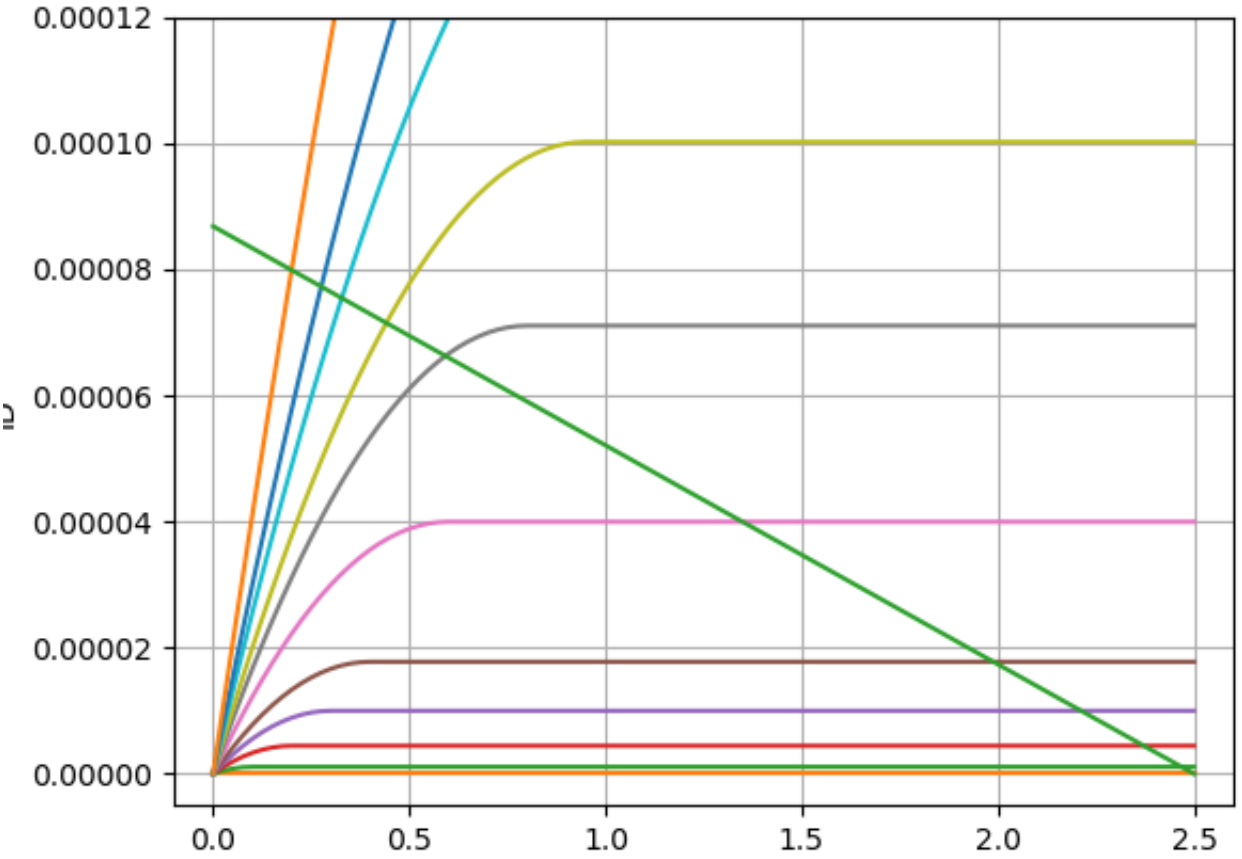
\includegraphics[width=0.5\linewidth]{img/carico_resistivo_cfre.png}
    \caption{Grafico di confronto inverter resistivo}
    
\end{figure}

\subsection{A carico saturato}

Bisogna fare attenzione in questo caso all'effetto body non trascurabile.


In saturazione: 
\begin{equation*}
    I_D = \frac{K_n}{2}(V_{GSL} - V_{TNL})^2
\end{equation*}

\begin{equation*}
    I_D = \frac{K_n}{2}(V_{DD} -V_{DS} -  V_{TNL})^2
\end{equation*}

Questo rappresenta l'arco di parabola in verde sul grafico.



\begin{figure}[htbp]
    \centering
    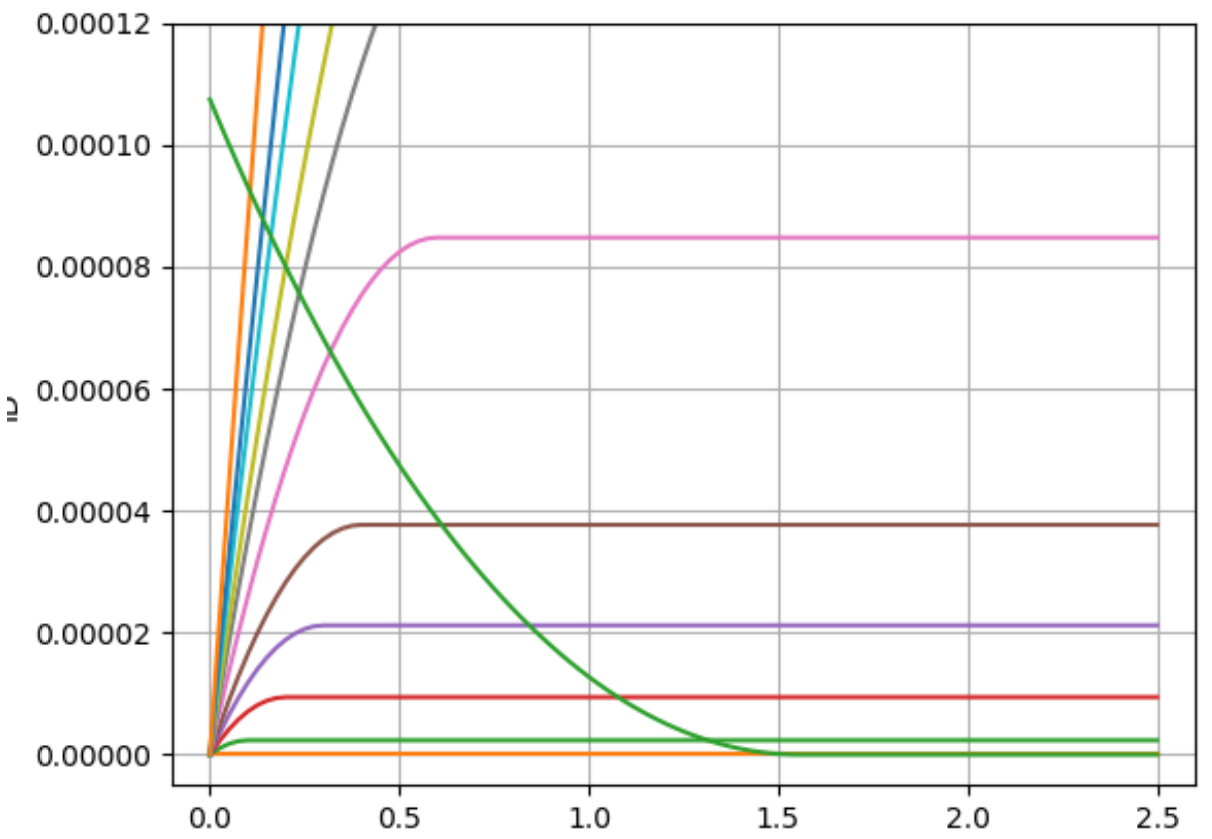
\includegraphics[width=0.5\linewidth]{img/a_saturamento_cfr.png}
    \caption{Grafico di confronto inverter a carico saturato}
\end{figure}


\newpage
\subsection{A carico deplation/svuotamento}

Vi sono due zone a seconda delle tensioni:


\begin{equation*}
    I_D = \frac{K_n}{2}(-V_{TNL})^2  \qquad \qquad \text{Per } V_{GSL} \leq V_{DSL}  + V_{TNL}
\end{equation*}

\begin{equation*}
    I_D = K_n\biggl(-V_{TNL} - \frac{V_{DSL}}{2}\biggl)V_{DSL}  \qquad \qquad \text{Per } V_{GSL} \geq V_{DSL}  + V_{TNL}
\end{equation*}



\begin{figure}[htbp]
    \centering
    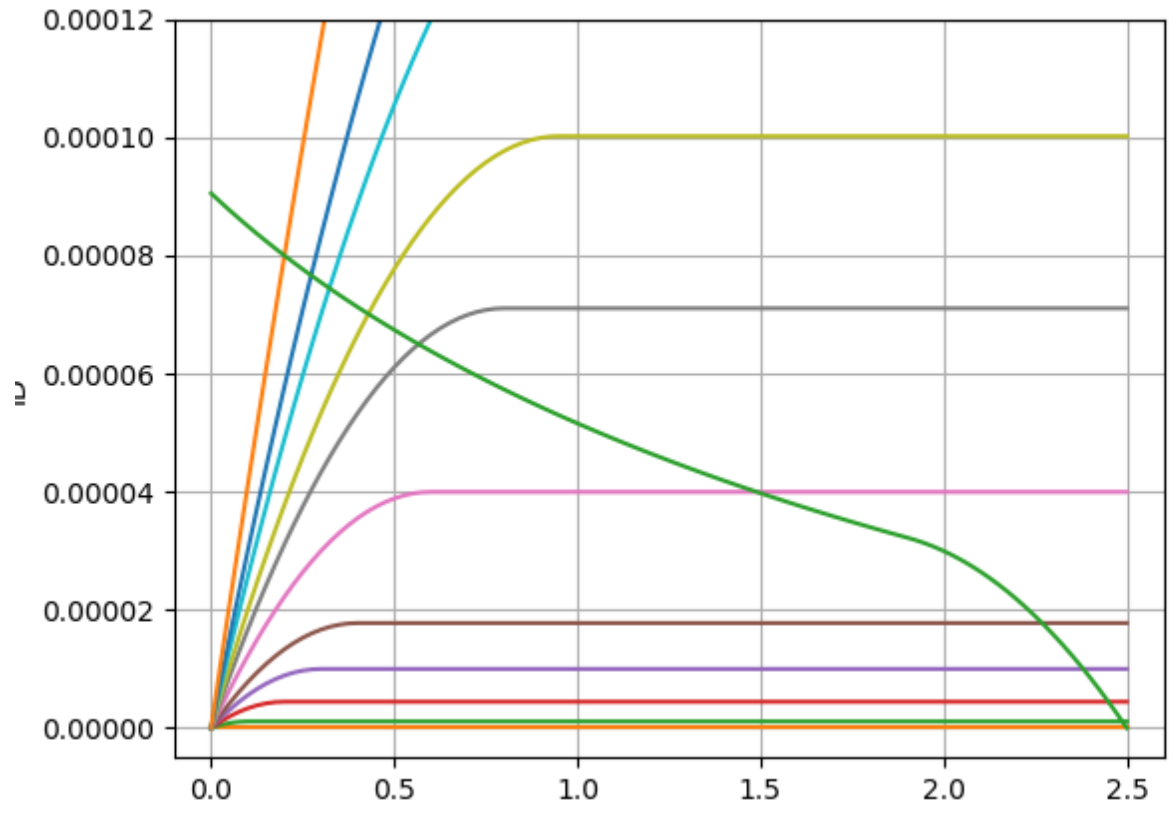
\includegraphics[width=0.5\linewidth]{img/deplation_cfr.png}
    \caption{Grafico di confronto inverter a svuotamento}
    
\end{figure}


\subsection{A carico pseudo nMOS}

Per quanto riguarda questo caso come carico ci ritroviamo la caratteristica di un transistore pMOS.

\begin{figure}[htbp]
    \centering
    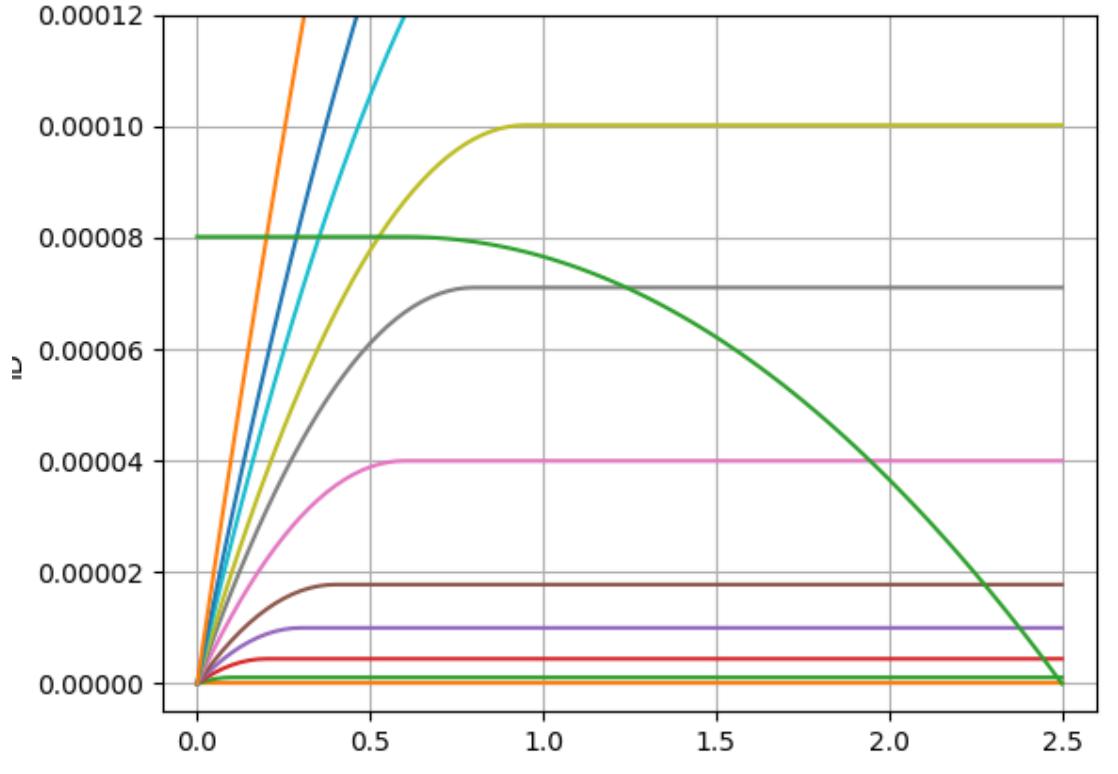
\includegraphics[width=0.5\linewidth]{img/pseudo_nnone.png}
    \caption{Grafico di confronto inverter pseudo nMOS}
    
\end{figure}


Questi grafici fanno vedere quanta corrente possono far scorrere i vari carichi. Quindi a parità di tutto il resto il pMOS conduce meglio la corrente soprattutto nel transitorio e potremmo caricare la capacità un po' più velocemente. Al netto anche dei margini di rumore leggermente inferiori al carico a svuotamento.


\newpage
\section{Impatto della saturazione di velocità}

Se i componenti sono più piccoli del micron entra in gioco anche la saturazione di velocità delle cariche, in particolare se il campo elettrico è al di sopra di $10^5\,V$.

Vediamo alcuni casi:

\begin{itemize}
    \item Se	il	campo	elettrico	è	troppo	alto,	la	velocità	dei	portatori	satura, supponiamo	$V_{DS} = V_{SAT} = 1.2 \,V$	sia	la	soglia	di	saturazione di velocità

    \item Per	il	pull	down	non	c’è	differenza
\end{itemize}

La saturazione ha effetto sul pull-up infatti la formula per definire la corrente tenendo presente la saturazione di velocità è la seguente:

\begin{equation*}
    I_D = K_n\biggl( \vgs - \vtn - \frac{V_{MIN}}{2}\biggl)V_{MIN}(1-\lambda V_{DS})
\end{equation*}

la formula è uguale alla zona triodo tranne che sostituiamo $V_{DS}$ con $V_{MIN}$:

\begin{equation*}
    V_{MIN} = min((\vgs - \vtn), V_{DS}, V_{SAT})
\end{equation*}

Rispettivamente il minimo tra: saturazione, triodo e saturazione di velocità.


\section{Impatto della saturazione di velocità}

\paragraph{Se usiamo un carico saturato:}


\begin{itemize}
    \item[] $V_{GS} - V_{TN} = 2.3 - 0.66 = 1.64\,V$
    \item[] $V_{DS} = 2.3\, V$
\end{itemize}

Occorre allora usare $V_{SAT} = 1.2 \,V$, in quanto interviene prima della saturazione normale del transistore

\begin{equation*}
    \frac{W}{L} = \frac{I_D}{K_n'(\vgs - \vtn - \frac{V_{SAT}}{2})V_{SAT}} = \frac{1}{1.56}
\end{equation*}

Confrontato con $1/68$, ottenuto	precedentemente, il	canale	deve	essere	leggermente	accorciato	per	compensare	la	perdita	
di	corrente	dovuta	alla	saturazione	di	velocità.



\paragraph{Se usiamo un carico svuotamento:}


\begin{itemize}
    \item[] $V_{GS} - V_{TN} = 0+0.94 =0.94\,V$
    \item[] $V_{DS} = 2.3 \,V$
\end{itemize}

$V_{GS} - V_{TN} < V_{SAT}$ non dobbiamo cambiare nulla.

\paragraph{Se usiamo uno pseudo nMOS:}



\begin{itemize}
    \item[] $V_{GS} - V_{TN} = 2.5 - 0.6 = 1.9\,V$
    \item[] $V_{DS} = 2.3\, V$
\end{itemize}

Occorre usare $V_{SAT} = 1.2 \,V$ ottenendo $\frac{W}{L} = \frac{1.28}{1}$. Confrontare	con	$1.11/1$	ottenuto	precedentemente, la larghezza	W	deve	essere	leggermente	aumentata	per	compensare	la	perdita	di	corrente	dovuta	alla	saturazione	di	velocità.


\paragraph{}
Con tecnologie moderne siamo sempre in saturazione di velocità, infatti inizialmente si parte sulla carta e poi si passa su Spice per confrontare i vari modelli con tecnologie di dimensioni diverse.

\chapter{Porte logiche}

Fino ad ora ci siamo focalizzati sull'invertitore con logia nMOS o anche chiamata logica a rapporto perché il livello delle uscite dipende dal dimensionamento del \textbf{pull-up} e del \textbf{pull-down} e a seconda li dimensioniamo abbiamo dei livello di uscita differenti. In particolare è il livello basso che viene particolarmente influenzato, quello alto arriva a $V_{DD}$ a meno che non si usi un carico saturato che vada in cut-off e dunque non porta più l'uscita a $V_{DD}$.

\paragraph{}
Con questa logica il pull-up viene è sempre acceso, e per portare all'uscita un valore basso si deve accendere il transistore sottostante per poter portare giù l'uscita, dopo un corretto dimensionamento.
\paragraph{}
Nulla vieta di fare il contrario: mettere un pull-down sempre attivo e un pull-up, pMOS, che viene controllato dall'ingresso.

Quando l'ingresso è altro non conduce, e il pull-down porta giù l'uscita.

Quando l'ingresso è basso, invece, è il pull-up che tira su l'uscita.

\begin{figure}[htbp]
    \centering
    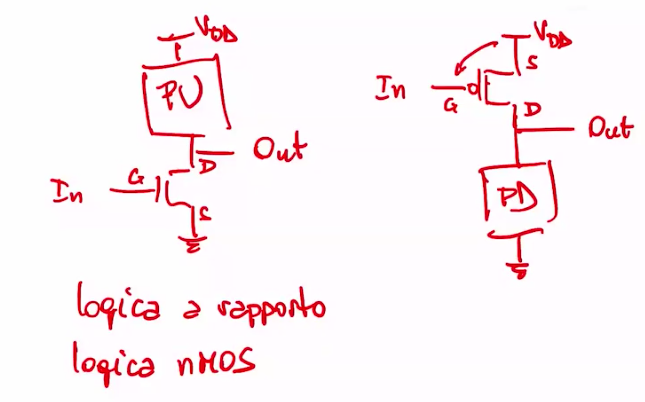
\includegraphics[width=0.5\linewidth]{img/logia_a_rapporto.png}
    \caption{Logia a rapporto}
    
\end{figure}

\paragraph{Come mai non si fa mai una logia a rapporto con un pMOS come pull-up?}

Ricordiamo che i pMOS e gli nMOS, data la stessa tecnologia, i transistori nMOS conducono meglio dei pMOS, questo perché la mobilità degli elettroni è più alta di quella delle lacune.

A parità di corrente che si vuole far passare l'nMOS è più piccolo, più corrente vogliamo più W deve essere grande.

Ma anche guardando la transconduttanza $K_N' = \mu_nC_{ox}^{''}\frac{W}{L}$, vediamo che troviamo un coefficiente moltiplicativo $\mu_n$, che riguarda la mobilità dei portatori, se più alta è la mobilità possiamo fare W più piccola, questo implica che si possono fare transistori più piccoli.


Dunque normalmente, per questa ragione, si cerca di utilizzare un nMOS. 

\paragraph{}
Per fare altre porte logiche possiamo constatare che il pull-up rimarrà sempre uguale, quello che varierà sarà il pull-down a seconda delle porte logiche da costruire.


\newpage
\section{Costruzione di porte logiche}
Per costruire le porte logiche fondamentali possiamo usare delle combinazione di transistori. In particolar modo si useranno transistori collegati in serie o in parallelo.


\begin{figure}[htbp]
    \centering
    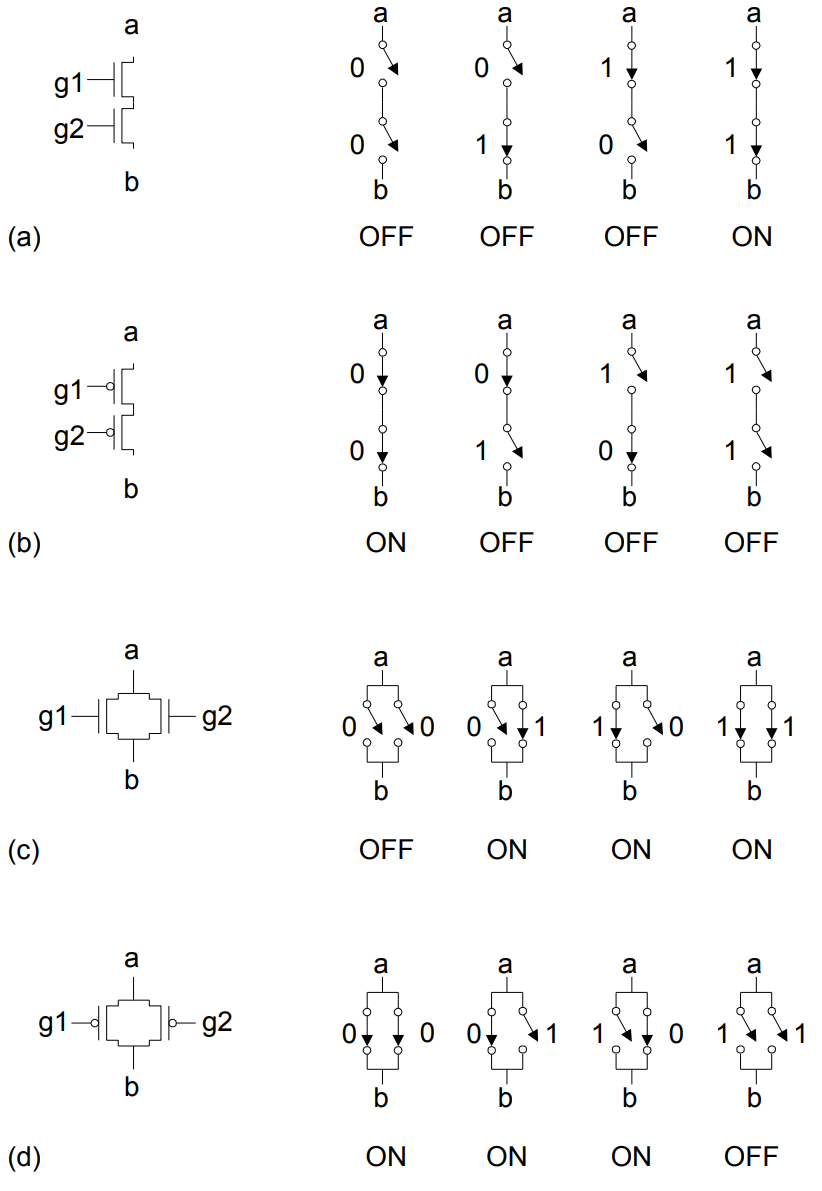
\includegraphics[width=0.5\linewidth]{img/and_or.png}
    \caption{Vari modi per costruire le porte AND, NAND, OR e NOR}  
    \label{and_or}
\end{figure}

Nel caso delle Figura \ref{and_or} nei casi a) nMOS e b) pMOS, i yransistori	in	serie	conducono	
se	e	solo	se	conducono	entrambi.
\paragraph{}
Nel caso delle Figura \ref{and_or} nei casi c) nMOS e d) pMOS, i transistori	in	parallelo	conducono	quando almeno un transistore è in conduzione.


\newpage
\section{Porta logica: NOR}

Vogliamo che l'uscita sia alta se e solo se entrambi gli ingressi sono bassi, altrimenti, vogliamo che l'uscita sia a zero quando almeno uno dei due ingressi è al livello alto. In questa maniera dovremo realizzare una costruzione parallela: il pull-down si deve attivare quando almeno un ingresso sia al livello alto.


\begin{figure}[htbp]
    \centering
    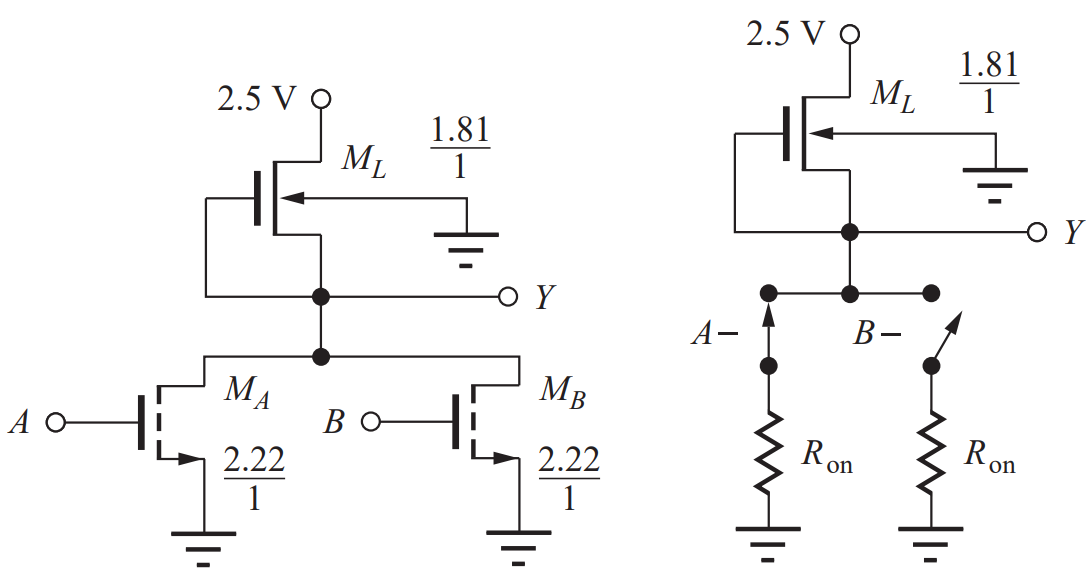
\includegraphics[width=0.5\linewidth]{img/NOR.png}
    \caption{Porta logia NOR}    
\end{figure}

\paragraph{NOTA: } la resistenza interna dei due transistori $R_{ON}$ deve essere inferiore alla resistenza del pull-up, per vincere il partitore e portare l'uscita a livello basso, definita a $0.2\,V$ o inferiore .
\paragraph{}

Affinché l'uscita sia al livello logico basso, dobbiamo dimensionare i due transistori di pull-down in modo tale che da soli siano in grado di tirare giù l'uscita. Il dimensionamento dunque è uguale a quello fatto per l'inverter: $\frac{W}{L} = \frac{2.22}{1}$.

\subsubsection{A quanto arriva l'uscita nel caso in cui $A = B = 2.5\,V$?}

Entrambi i transistori conducono e si trovano in zona triodo, mentre il pull-up si trova in zona si saturazione ($V_{GS} = 0V$ e $V_{DS}$ è alta sicuramente $V_{DS} \leq (2.5 - 0.2)\,V$).


Quindi per trovare quanto vale l'uscita ci basta uguagliare le due equazioni:

\begin{equation*}
    2K_n'2.22\biggl(\vgs - \vtn - \frac{\vds}{2}\biggl)\vds = \frac{K_n'}{2}1.81(V_{GSL} - V_{TNL})^2
\end{equation*}

dove:

\begin{itemize}
    \item $V_{TN}$, supponiamo che non ci sia effetto body e la uguagliamo a $0.6\,V$.
    \item $V_{GSL}$ questa risulta essere zero, per costuzione del circuito
    \item $V_{TNL}$ dovremmo considerare l'effetto body, $V_{TNL} = V_{TO} + \gamma\sqrt{V_{DS} + 2\phi_F} - \sqrt{2\phi_F}$
    \item L'equazione a sinistra viene moltiplicata per un fattore 2 perché la corrente, essendo i sue transistori uguali, si splitterà in due.
\end{itemize}

\paragraph{Ipotesi: } mettiamo una $V_{TNL}^2 = 0.94$, cerchiamo di indovinarla. Sicuramente ci sarà un errore ma non importa in quanto di per se, già il modello che usiamo contiene degli errori ed ulteriori semplificazioni possono aiutare al posto di risolvere l'equazione con due radici non comode da gestire.

\begin{equation*}
    8.88\biggl(1.9  - \frac{\vds}{2}\biggl)\vds = 1.81\cdot0.94
\end{equation*}

\begin{equation*}
    4.44\vds^2 - 16.872\vds + 1.7 = 0
\end{equation*}
\begin{equation*}
    \vds = 0.103 \,V
\end{equation*}

Quest'ultima era $0.2\,V$, con due pull-down scende di quasi la metà.

\newpage
\section{Porta logica: NAND}

Essendo la NAND non attiva se e solo se entrambi gli ingressi sono alti, il pull-down deve portare l'uscita a zero solo quando entrambi gli ingressi sono alti e per questo utilizzeremo due transistori in serie. Se uno dei due ingressi è interdetto, la corrente non va a massa e il pull-up porta l'uscita al livello alto.

\paragraph{}
Questi due resistori devono portare una corrente di $80\,\mu A$, come definito dalle specifiche, però sono in serie e la tensione, essendo i due transistori uguali, si ripartisce circa a metà. Per far in modo che portino la stessa corrente di prima dovremo fare dei transistori più grossi (in prima approssimazione dovranno essere grossi il doppio: $W/L = 4.44$).

\paragraph{Come mai diventa più grosso?} Come per i condensatori in parallelo, o i resistori in serie, le lunghezze dei due transistori si sommano, formando quindi una lunghezza doppia, e per ottenere sempre lo stesso rapporto, che ci garantisce che possa passare tanta corrente quanta le specifiche dicono, dobbiamo aumentare W. Aumentiamo del doppio L dobbiamo aumentare del doppio anche W per mantenere il medesimo rapporto $W/L$.

\begin{figure}[htbp]
    \centering
    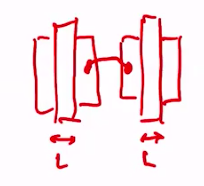
\includegraphics[width=0.25\linewidth]{img/trans, serie.png}
    \caption{Transistori in serie}    
\end{figure}
 
\paragraph{Se fossero in parallelo: } i transistori in questo caso è come se fosse W doppia, quindi L la facciamo molto piccola, il quale implica che due transistori in parallelo conducano molto bene.

\begin{figure}[htbp]
    \centering
    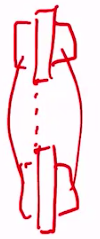
\includegraphics[width=0.13\linewidth]{img/trans_parall.png}
    \caption{Transistori in parallelo}    
\end{figure}

\newpage
Ritornando a noi, dimensionandoli in questa maniera siamo sicuri che riescano a trasportare $80\,\mu A$. 

Tutto questo in prima approssimazione perché:
\paragraph{}
Non siamo sicuri che la tensione si ripartisca esattamente a metà, infatti il source di B non è collegato a massa, bensì è collegato al drain di A, questo provocare il fenomeno dell'effetto body per il transistore B. Questo effetto gli fa alzare la tensione di soglia.

Questo comporta che:
\begin{itemize}
    \item $V_{GSMA} = V_{DD}$ perché il source è collegato a massa e l'effetto body non si presenta;
    \item $V_{GSMB} \neq V_{DD}$ perché il source è collegato al drain di $M_A$ e per questo si presenta l'effetto body il quale innalza la tensione di soglia. 
\end{itemize}

In particolare $V_{GSMB}$ è in una situazione meno favorevole di $M_A$ in quanto conduce di meno perché ha una $V_{GSMA}$ più bassa e ha una tensione di soglia più alta, questo comporta che $M_B$ dovrà essere più grosso di $M_A$ per compensare la differenza di conduzione che vi è tra i due.

\newpage
\section{Dimensionamento dei transistori in fase di conduzione}

Supponiamo che $V_0$ si divida esattamente in due, dunque su ogni transistore, se l'uscita va a $0.2\,V$, cadrà esattamente $0.1\,V$: $V_{DS} = 0.1\,V$, si entrambi. Questo per semplificare, sempre dato dal fatto che già il modello non è preciso, qualche semplificazione possiamo farcela per fare i conti in maniera più agile.

\subsection{Per $M_A$}

Le cose sono sempre come prima, è cambiata solo la $V_{DS}$ si è dimezzata:

\begin{equation*}
    K_n'\biggl(\frac{W}{L}\biggl)_A\biggl(V_{GSA} - V_{TNA} -\frac{V_{DSA}}{2}\biggl)V_{DSA} = I_D = 80\, \mu A
\end{equation*}

dove

\begin{itemize}
    \item $V_{GSA} = 2.5\,V$;
    \item $V_{TNA} =0.6\,V $;
    \item $V_{DSA} = 0.1\,V$
\end{itemize}

\begin{equation*}
    \biggl(\frac{W}{L}\biggl)_A = \frac{80}{100\big(2.5 - 0.6 - \frac{0.1}{2}\big)0.1} = 4.32
\end{equation*}

Vediamo che non viene esattamente $4.44$ bensì un po' meno, questo è anche dovuto al fatto che abbiamo fatto i conti in maniera un pelo più oculata.


\subsection{Per $M_B$}

La tensione di soglia è alterata, quindi dovremmo usare la formula che tiene conto dell'effetto body:

\begin{equation*}
    V_{TNB} = V_{TN} + \gamma \big(\sqrt{V_{DSA} + 2\phi_F} - \sqrt{2\phi_F}\big) = 0.63\,V
\end{equation*}

Per determinare il  valore di $V_{DSA}$ entra in gioco la semplificazione detta pocanzi: $0.1\,V$. 

Anche questo transistore si trova in zona triodo, pertanto:

\begin{equation*}
    K_n'\biggl(\frac{W}{L}\biggl)_B\biggl(V_{GSB} - V_{TNB} -\frac{V_{DSB}}{2}\biggl)V_{DSB} = I_D = 80\, \mu A
\end{equation*}

dove

\begin{itemize}
    \item $V_{GSB} = 2.4\,V$;
    \item $V_{TNB} =0.63\,V $;
    \item $V_{DSB} = 0.1\,V$
\end{itemize}


\begin{equation*}
    \biggl(\frac{W}{L}\biggl)_A = \frac{80}{100\big(2.4 - 0.6 - \frac{0.1}{2}\big)0.1} = 4.65
\end{equation*}

\paragraph{}
Dunque il transistore più in altro risulterà essere più grosso.

\newpage

\section{AND}
Il pull-down deve essere attivo quando almeno uno degli ingressi si trova a zero, quindi risulterà essere una NAND con una negazione in cascata.

Infatti la AND, con questa logica, non è possibile farla sul pull-down perché è fatto con nMOS e se gli ingressi sono a zero, si mettono in interdizione e il circuito ritorna il valore alto: $V_{DD}$.

Dunque una logia fatta nel modo in cui l'abbiamo vista è \textbf{sempre invertente}, ecco anche perché è possibile utilizzare un inverter dopo la porta logica NAND.

\paragraph{}
La AND costruita in questo modo sarà costituita da 5 transistori e sarà anche più lenta dovuto al fatto che vi è anche un inverter. Dunque conviene sempre usare porte invertenti piuttosto che usare le porte non invertenti.

Infatti un circuito a due livelli, studiato nel corso Reti Logiche, costituito da un livello di AND seguito in seguito da porte OR, non verrà mai fatto con porte non invertenti, bensì con porte invertenti perché sono più veloci, portando al medesimo risultato.

\begin{figure}[htbp]
    \centering
    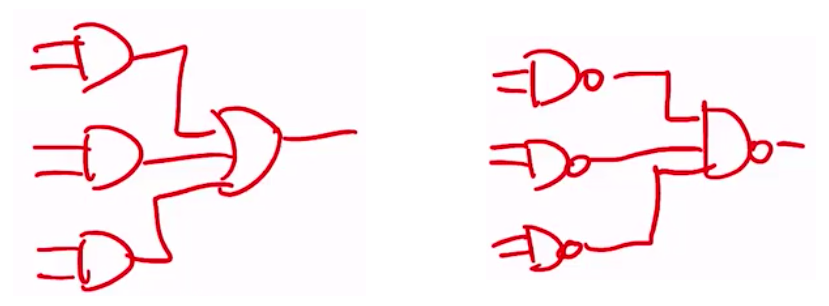
\includegraphics[width=0.6\linewidth]{img/circ_due_livelli.png}
    \caption{Circuito a due livelli}    
\end{figure}

Nelle NOR i circuiti vanno ancora più veloce perché i transistori sono inseriti in parallelo, oppure più piccole comunque.

Infatti una volta, quando si utilizzava questa logica a rapporto, si facevano tutti i circuiti con le NOR, per intenderci si sintetizzano gli zeri nelle mappe di Karnaugh.

\newpage
\section{Porte	logiche	complesse}

Non c'è bisogno di fare circuiti solo con NAND e NOR, ma basta mettere nel pull-down la combinazione adatta per ottenere un uscita desiderata, possiamo dunque costruire funzioni complesse direttamente nel pull-down.


\paragraph{Esempio: } Y = (A+BC+BD)' = (A+B(C+D))'

\begin{figure}[htbp]
    \centering
    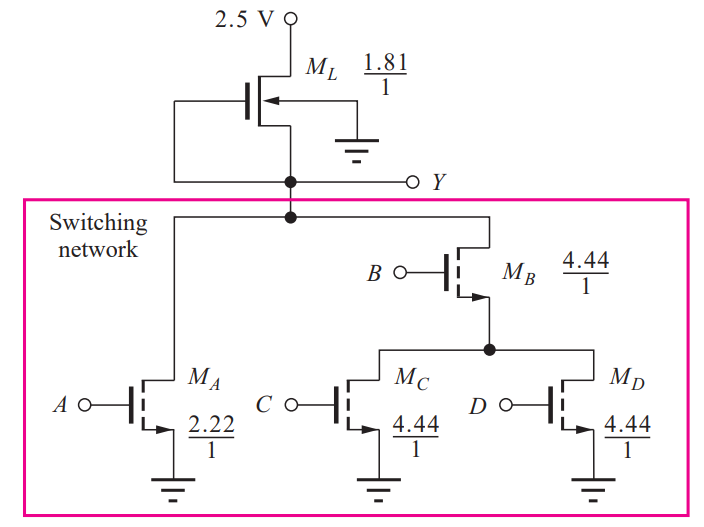
\includegraphics[width=0.5\linewidth]{img/funz_coplesse.png}
    \caption{Esempio di funzione complessa}    
\end{figure}

\paragraph{NOTA:} nella parte di destra si sarebbe potuto benissimo mettere C e D sopra, al posto di B, e mettere quest'ultimo al posto dei transistori C e D. Il problema sorge dal fatto che vi è l'effetto body, dove nel caso della figura si ha solo su B, nel caso in cui volessimo invertire l'effetto si presenterebbe su due transistori, C e D, al posto che solamente su B.


\paragraph{}
Il dimensionamento è sempre fatto nei casi peggiori: 

\begin{itemize}
    \item se solo A attivo, deve potere portare l'uscita bassa (NOT);
    \item se solo B e C attivi, assieme, devono portare l'uscita bassa (NAND);
    \item se solo B e D attivi, assieme, devono portare l'uscita bassa (NAND).
\end{itemize}

\newpage
\section{Tempistiche}

Andiamo a vedere ora le tempistiche di questi circuiti, in particolare che metriche ci interessano dal punto di vista delle tempistiche? Dal momento in cui cambia l'ingresso, quanto impiega l'uscita a cambiare?

Questo è essenziale per determinare la velocità di un circuito scandito dal clock: nel tempo di salita/discesa del clock la logia deve aver calcolato il risultato, ovvero deve aver raggiunto un uscita stabile (vedi tempo di Set-Up e tempo di Hold).


\subsection{Comportamento dinamico: i ritardi}

\subsubsection{Ritardo di propagazione}
Tempo	che	intercorre	tra	
la	transizione	dell’ingresso	
e	quella	dell’uscita. Di	norma	i	ritardi	sono	
diversi	a	seconda	della	
transizione.

Per determinarlo si osserva quando la transizione  passa per il 50\% della tensione totale. Questo tempo potrebbe anche venire influenzato dal secondo tipo di ritardo: il tempo di rise e fall.

\paragraph{}
Questa metrica ci dice quanto \textbf{veloce} va il circuito.


\subsubsection{Ritardo di salita e discesa (rise e fall)}

Tempo	che	impiega	
l’uscita	a	passare	dal	10\%	
al	90\%	(o	viceversa).

Non prediamo in considerazione la derivata in quanto essendo molto bassa all'inizio comporterebbe gradi errori di tempistiche.


\begin{figure}[htbp]
    \centering
    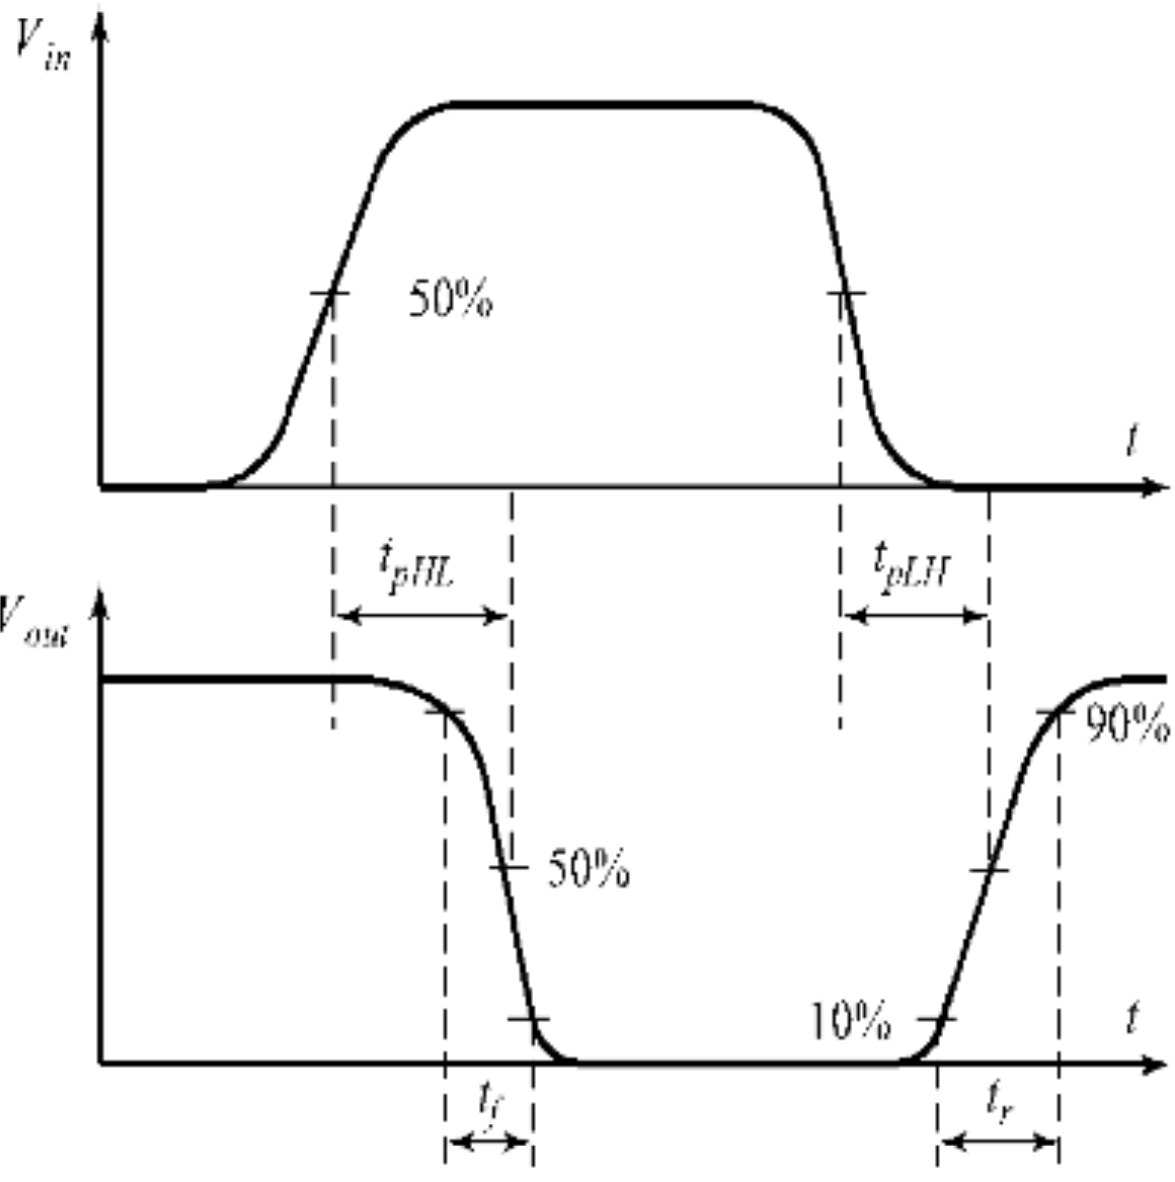
\includegraphics[width=0.5\linewidth]{img/ritardi.png}        
\end{figure}

Questo ritardo è noto	come	\textbf{slew rate}, questa metrica ci dice quanto velocemente cambiano entrambi i fronti.

\newpage
\subsection{Capacità nel transistor MOS}

I ritardi, l'uscita che non segue immediatamente l'ingresso, sono insiti nel circuito del transistore, in quanto il suo gate si comporta proprio un \textbf{condensatore} a piatti piani paralleli con differenti capacità:

\begin{itemize}
    \item tra gate e canale;
    \item tra gate e source/drain (overlap);
    \item capacità dei diodi (non lineare);
    \item capacità non lineari, che dipendono anche dalla zona di funzionamento.
\end{itemize}


\begin{figure}[htbp]
    \centering
    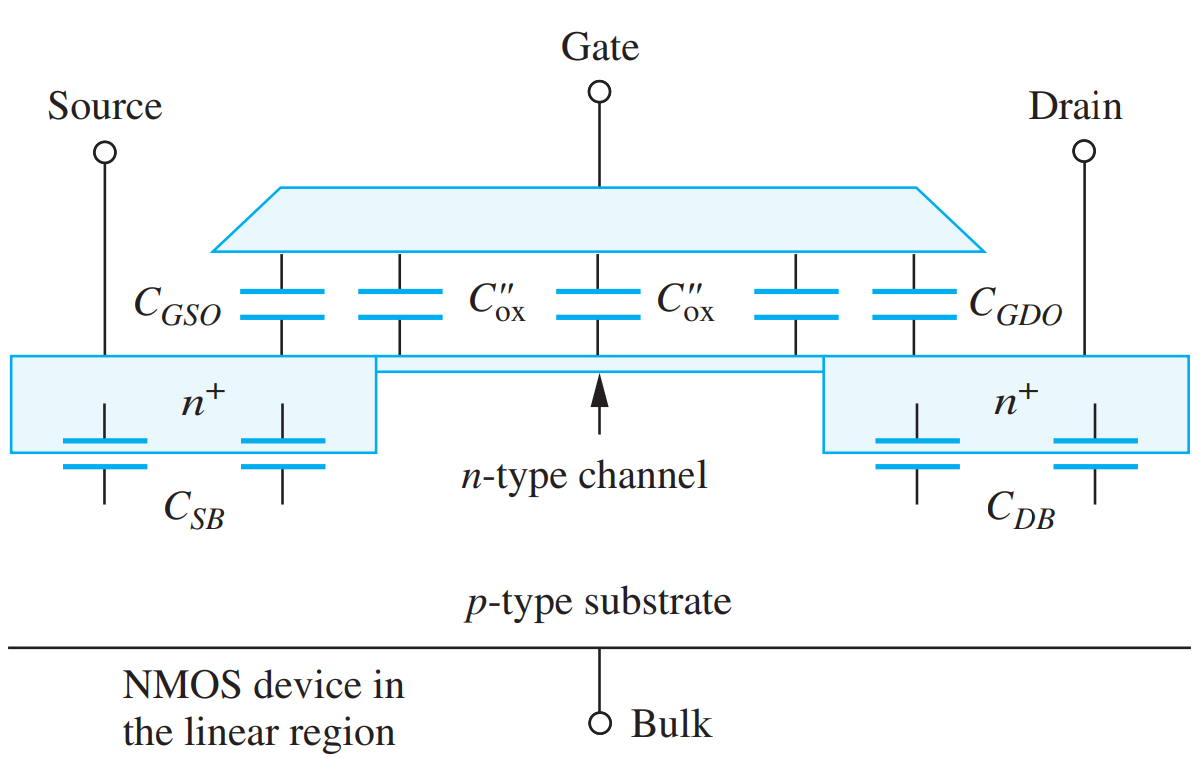
\includegraphics[width=0.5\linewidth]{img/cond_a_piatti.png}
    \caption{Capacità lineari e non in un transistore}
    
\end{figure}

La tensione sul condensatore non può cambiare istantaneamente, perché servirebbe una potenza infinita e dunque un picco di corrente infinita, tutto questo non è possibile e dunque la tensione cambia in maniera graduale.

\subsection{Transitorio dell'invertitore a carico resistivo}

Calcoliamo, nel circuito più semplice visto fino ora, quanto tempo impiega il gate a valle a caricarsi. Poniamo inizialmente $V_I = V_{DD} = 2.5\,V$ e l'uscita $V_L = 0.2\,V$, successivamente, a $t=0\,s$ vi è una transizione sull'ingresso infatti ora $V_I = V_L = 0.2\,V$. Figura \ref{transitorio} a).

\paragraph{}
Per $t<0$ l'uscita valeva $0.2\,V$ quindi il condensatore a valle aveva una differenza di potenziale ai suoi capi di $0.2\,V$.

\paragraph{}
Per $t \leq 0$ il gate del transistore va a $0.2\,V$ e l'uscita viene portata a $2.5\,V$ dal pull-up e il condensatore inizia a caricarsi. Figura \ref{transitorio} b).

Si caricherà secondo lo stesso principio di caricamento di un circuito RC: con la carica esponenziale.

\begin{equation*}
    V_O = V_2 - (V_2 - V_1)e^{-\frac{t}{RC}}
\end{equation*}

dove:

\begin{itemize}
    \item $V_1 = 0.2\,V$
    \item $V_2 = 2.5\,V$
    \item R la sappiamo dato che il circuito lo abbiamo progettato
    \item C lo sappiamo dato che è la somma di tutte le capacità dei gate a valle
\end{itemize}

\begin{figure}[htbp]
    \centering
    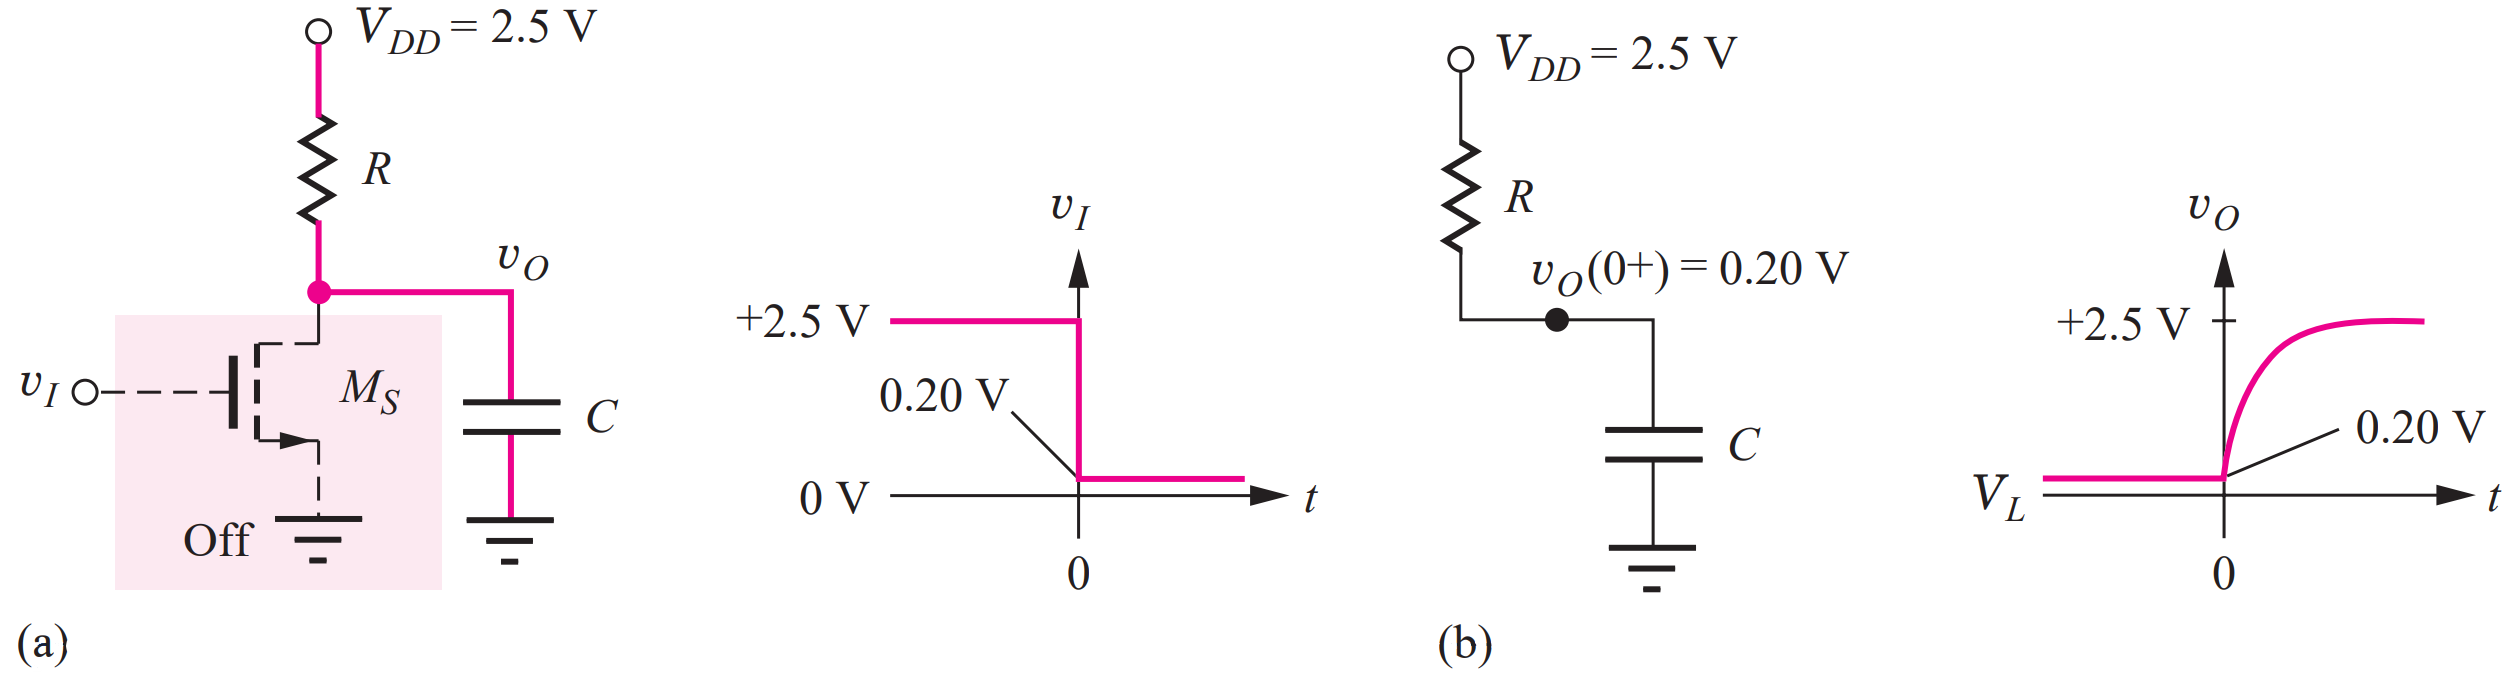
\includegraphics[width=1\linewidth]{img/inver_trans.png}
    \caption{transizione in salita}
    \label{transitorio}
\end{figure}


\subsection{Tempo di salita}
Dobbiamo vedere quando l'uscita passa tra	il	10\%	e	il	90\%	del	range	di	valori (non è $2.5\,V$, bensì $(2.5-0.2)\,V$):

\begin{itemize}
    \item $10\%: V_1 + 0.1(V_2-V_1) = 0.2+0.1(2.5-0.2) = 0.43\,V$
    \item $90\%: V_1 + 0.9(V_2-V_1) = 0.2+0.9(2.5-0.2) = 2.27\,V$
\end{itemize}

\begin{equation*}
    0.43 = 2.5 - 2.3e^{-\frac{t}{RC}} \qquad\qquad t_1 = -RC\ln(0.9)
\end{equation*}
\begin{equation*}
    2.27 = 2.5 - 2.3e^{-\frac{t}{RC}} \qquad\qquad t_1 = -RC\ln(0.1)
\end{equation*}


\begin{equation*}
    t_r = t_2 - t_1 = 2.22RC
\end{equation*}

Quindi in questo caso il tempo di salita è un multiplo della costante di tempo $\tau$, e la costante è appunto $2.22$.

\subsection{Tempo di propagazione}
Questo caso e più semplice, mi basta trovare quanto tempo impiega per passare a metà, 50\%, della sua escursione massima.


\begin{itemize}
    \item[] $50\%: V_1 + 0.5(V_2-V_1) = 0.2+0.5(2.5-0.2) = 1.35\,V$
\end{itemize}
\begin{equation*}
   1.35 = 2.5 - 2.3e^{-\frac{t}{RC}} \qquad\qquad t_1 = -RC\ln(0.5)
\end{equation*}

Quando è che passa per il valore cercato? A tempo $t=0\,s$ perché abbiamo presupposto che cambi istantaneamente: all'istante 0 passerà per tutti i valori.

\begin{equation*}
    t_{PLH} = t1 = 0.69RC
\end{equation*}

Dunque l'inverter andrà tanto più in fretta, tanto più C è piccola (transistori a valle più piccoli e pochi così che la capacità non cresca troppo). Il tempo di calcolo è fortemente dipendente anche dalla topologia del circuito e non solamente dalla porta logica in se. 


\paragraph{}

Un altro parametro che possiamo cambiare è R, tanto più piccola è R tanta più corrente può passare (al limite è un filo) e tanto più in fretta carica il/i condensatore/i a valle.

La R però la abbiamo ricavata dalle specifiche di consumo totale diviso il numero di porte (con stima della metà) accese e da li abbiamo ricavato quanta doveva essere la corrente che fluiva su ogni resistenza e attraverso la legge di Ohm ci siamo ricavati il valore della resistenza. Quindi va da se che se diminuiamo R passa più corrente e questa porterà ad un consumo maggiore a fronte di un miglioramento di velocità.


\paragraph{Esempio}

\begin{enumerate}
    \item Sia $R=28.8\, K\Omega$ e $C = 0.2\,pF$ i tempi saranno rispettivamente:
    \begin{itemize}
        \item[] $t_r = 2.2RC = 12.7\, ns$
        \item[] $t_{PLH} = 0.69RC = 3.97 \,ns$
    \end{itemize}

    \item Sia $R=28.8 K\Omega$ e $C = 0.5\,pF$ i tempi saranno rispettivamente:
    \begin{itemize}
        \item[] $t_r = 2.2RC = 31.7\, ns$
        \item[] $t_{PLH} = 0.69RC = 9.94\, ns$
    \end{itemize}
\end{enumerate}

Facendo un rapido calcolo notiamo che sono tempistiche davvero enormi se confrontati con i tempi di clock odierni: supponiamo un clock di $4Ghz$, il completamento di un operazione deve essere effettuato entro 

\begin{equation*}
    \frac{1}{4\cdot 10^{9}} = 2.5\cdot10^{-10}s = 0.25\cdot10^{-9}\,s 
\end{equation*}

stiamo parlando di più di un ordine di grandezza di differenza.



\subsection{Transitorio in discesa}

In questo caso è più complicato perché ad agire è il transistore e non il resistore ma questo rimane ugualmente.

\paragraph{}
Inizialmente l'ingresso è a $0.2\,V$  e l'uscita si trova a $V_{DD}$, al tempo $t>0$ l'ingresso si trova a $V_{DD}$ e l'uscita deve scendere fino a $0.2\,V$. Al tempo $t>0$ il transistore si trova in zona di saturazione perché la $V_{DS}$ è alta il quale inizia a scaricare la capacità, dunque il valore del drain inizia ad abbassarsi perché la capacità viene scaricata dal transistore.

In questa fase la scarica è costante, quasi lineare; non passa nessuna corrente per R in quanto vi è la medesima differenza di potenziale.

\paragraph{}
La tensione ai capi di C scende fintantoché scende ad una tensione di soglia sotto il gate, $V_O < G_{GS} - V_T$, e dunque entra in zona triodo.


In questa fase la scarica non è più costante e inizia a scendere anche quella del transistor e il condensatore si scarica sempre meno in fretta, in più vi è anche la resistenza R da tenere in considerazione. Infatti man mano che scende la tensione sul drain vi è corrente che passa per la resistenza la quale aumenta più il condensatore viene portato a massa.

\paragraph{}
Dunque la maggior parte della corrente passa attraverso la resistenza e non dal condensatore il quale fatica a scaricare le cariche depositate sulla capacità, infatti quando arriviamo a $0.2V$ (specifica di progetto) ai capi di C, tutta la corrente che passa per il transistore è passata prima da R. Infatti più in basso di $0.2V$ C non arriva.

\begin{figure}[htbp]
    \centering
    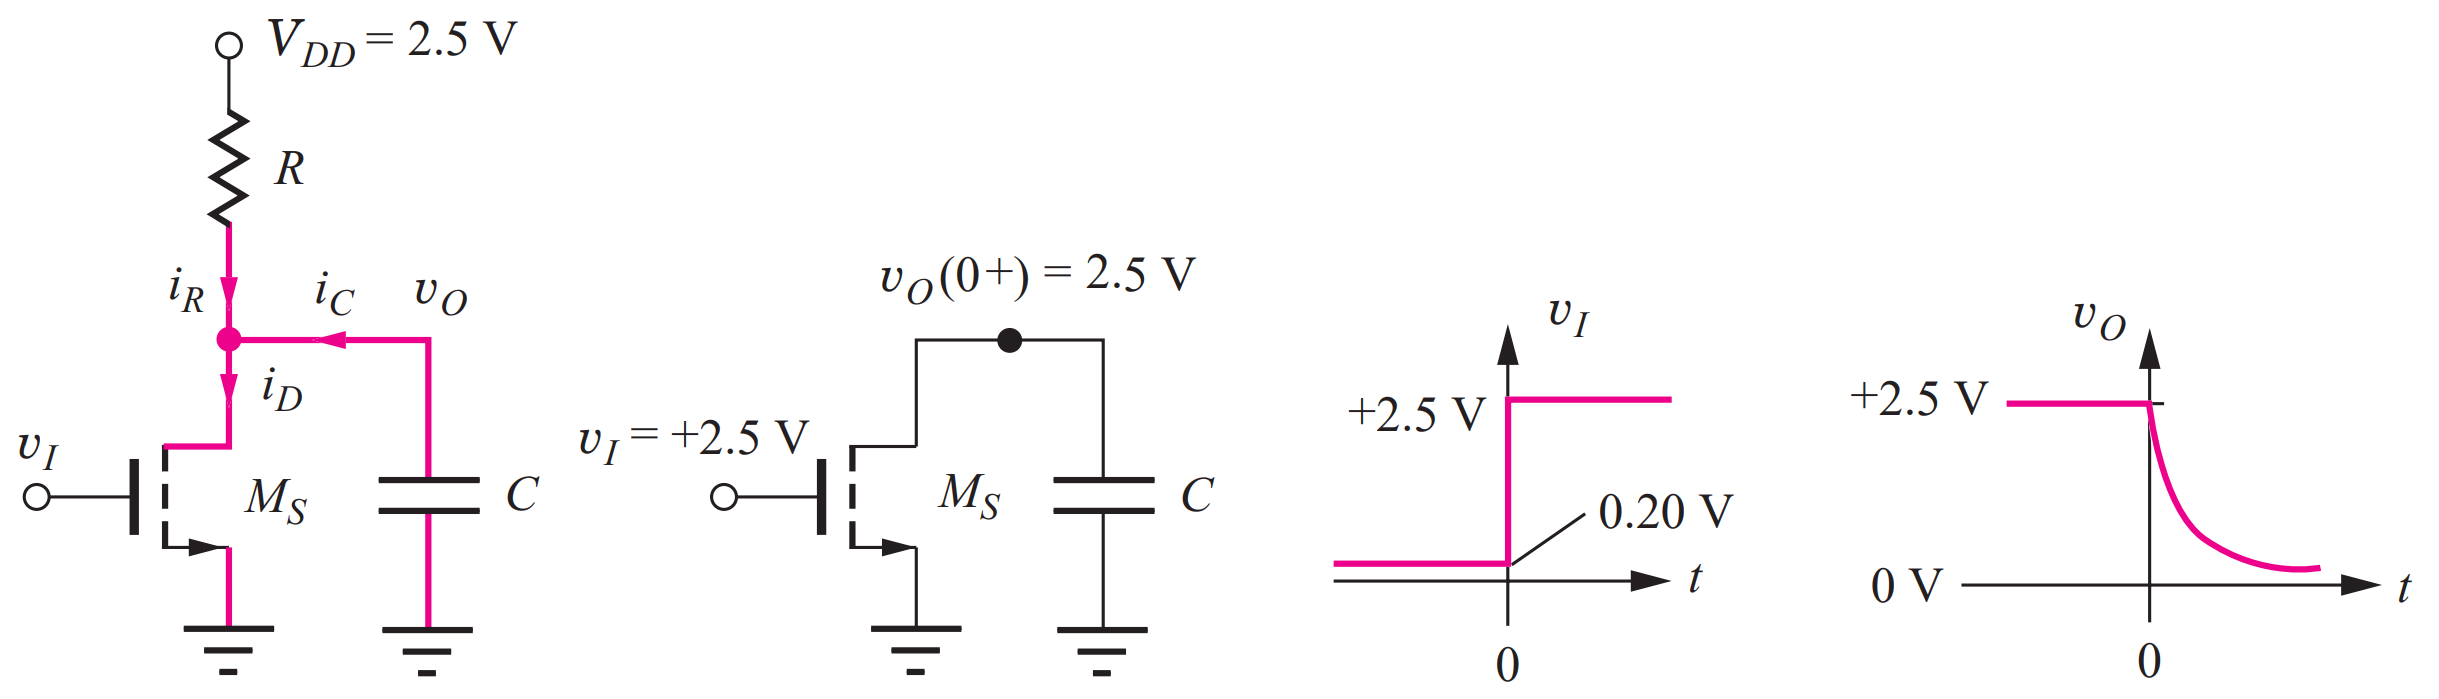
\includegraphics[width=1\linewidth]{img/trans_discesa.png}
    \caption{Transizione in discesa}    
\end{figure}


\subsection{Transitorio complesso}

Il transitorio passa per diverse regioni di funzionamento:

\begin{itemize}
    \item Comincia	in	zona	di	saturazione,	perché la	tensione	di	uscita	inizialmente	a	$2.5	V$ non	può	cambiare	istantaneamente;
    \item Si	segue	quindi	la	caratteristica	fino	ad arrivare	sulla	retta	di	carico
\end{itemize}


\begin{figure}[htbp]
    \centering
    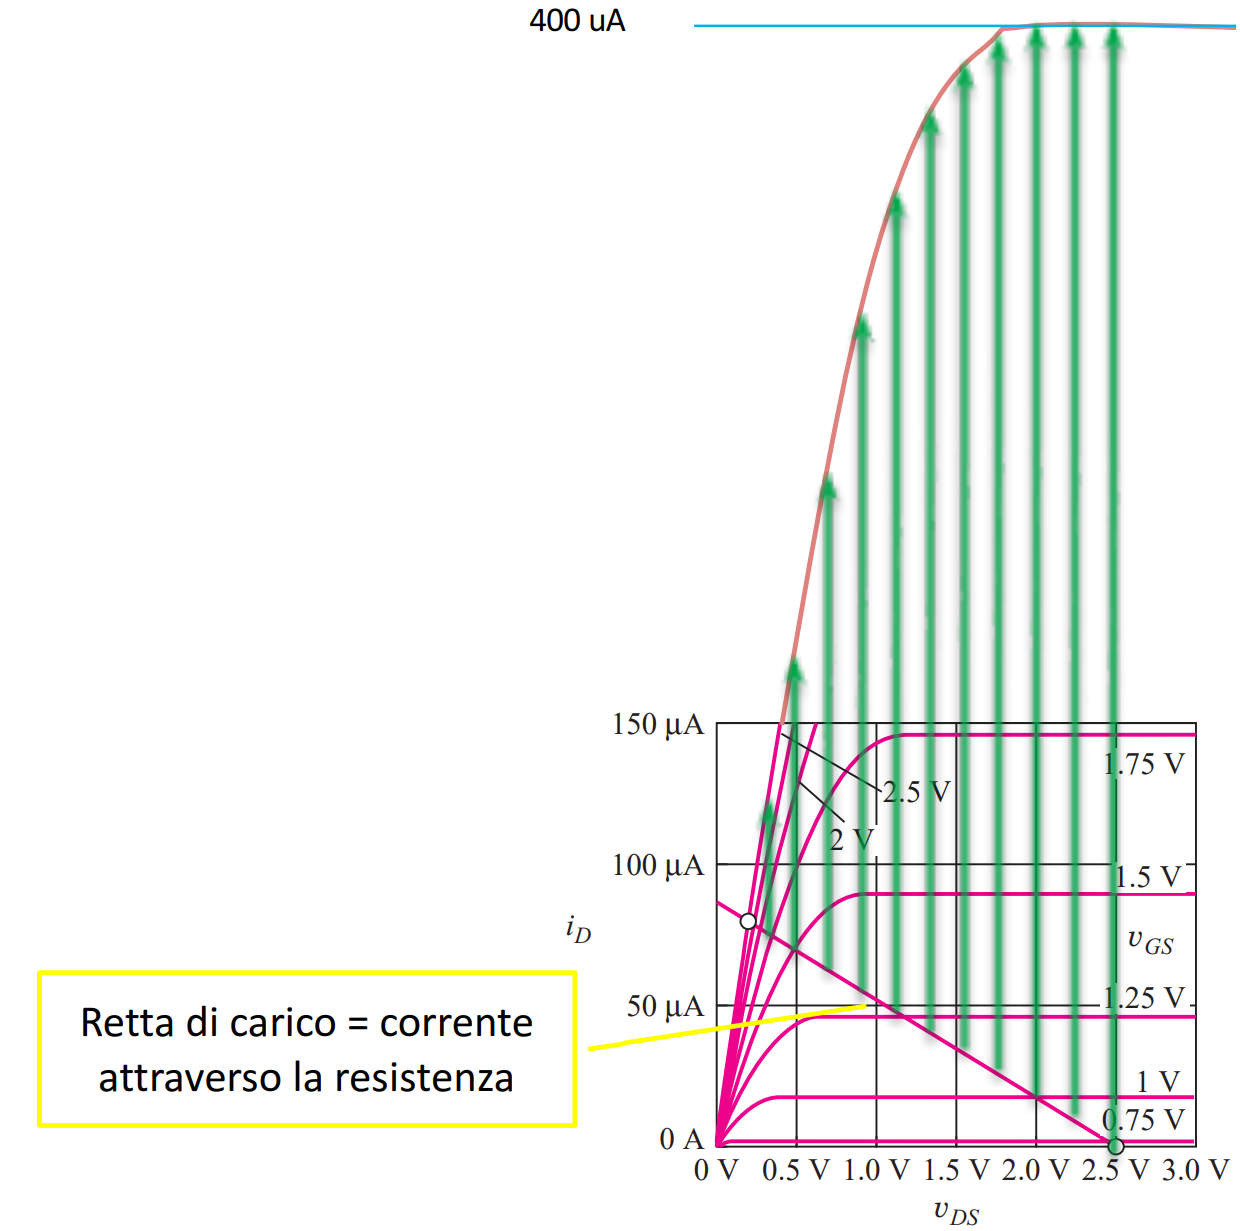
\includegraphics[width=0.5\linewidth]{img/retta_car_res.png}
    \caption{Transitorio complesso}
    \label{retta_carico}
\end{figure}

La freccia in verde raffigura la corrente che serve per scaricare la capacità C, si vede che scende e anche che non è particolarmente lineare perché aumenta la corrente sulla resistenza.

\subsubsection{Transitorio	in	discesa}

I conti sono decisamente più complessi, infatti una prima semplificazione possiamo considerare che la corrente che passa attraverso la resistenza è piccola, ce la dimentichiamo, tanto il modello non è preciso tanto vale semplificare al massimo.

\paragraph{}
Per approssimare il valore della resistenza senza fare innumerevoli conti possiamo determinare la resistenza da utilizzare partendo da $R_{on}$, resistenza che vediamo quando $V_{DS}$ tende a zero in Figura \ref{retta_carico}, corretta per un fattore correttivo.

\begin{equation*}
    I_D = K-n(V_{GS} - V_T)V_{DS}   \qquad\qquad \text{Se $V_{DS}$ è  bassa}
\end{equation*}

\begin{equation*}
    R_{on} = \frac{1}{K_n(V_{GS} - V_T)}
\end{equation*}

Per determinare R si utilizza un fattore correttivo del valore di $1.7$:
\begin{equation*}
    R = 1.7 R_{on}
\end{equation*}


\begin{equation*}
    t_{f} = 2.2(1.7R_{on})C = 3.7R_{on}C
\end{equation*}

\begin{equation*}
    t_{PHL} = 0.69(1.7R_{on})C = 1.2R_{on}C
\end{equation*}

Prendiamo queste due ultime espressioni per calcolare il tempo di salita e discesa HL.


\paragraph{Esempio}

\begin{itemize}
    \item Sia $R=28.8\, K\Omega$ e $C = 0.5\,pF$ i tempi saranno rispettivamente:
    \item $K_m = 2.22(100\,\mu A/V^2) = 222\,\mu A/V^2$
    \begin{itemize}
        \item[] $t_r = 2.2RC = 31.7\, ns$, calcolo precedente
        \item[] $t_{PLH} = 0.69RC = 9.94\, ns$, calcolo precedente
    \end{itemize}
\end{itemize}

Calcoliamo ora il tempo di discesa:


\begin{equation*}
    R_{on} = \frac{1}{(222(2.5-0.6))} = 2.37\,K \Omega
\end{equation*}
Da notare che è molto più piccola di R, perché il pull-down deve essere molto piccola, altrimenti il partitore non tira giù l'uscita
\begin{itemize}
    \item[] $t_r = 3.7R_{on}C = 4.39\, ns$
    \item[] $t_{PHL} = 1.2R_{on}C = 1.42\, ns$
\end{itemize}


La media: 

\begin{equation*}
    t_p = (t_{PHL} + t_{PLH})/2 = 5.68\,ns
\end{equation*}

\paragraph{Osservazione: } il comportamento del circuito è molto asimmetrico ed è dovuto	al	fatto	che	il	pull	down	deve	avere	una	resistenza	in	
conduzione	molto	minore	del	carico	per	raggiungere	un	valore	
di	$V_L$ sufficientemente	basso.



La	simulazione	con	Spice	conferma	i	risultati	ottenuti:

\begin{figure}[htbp]
    \centering
    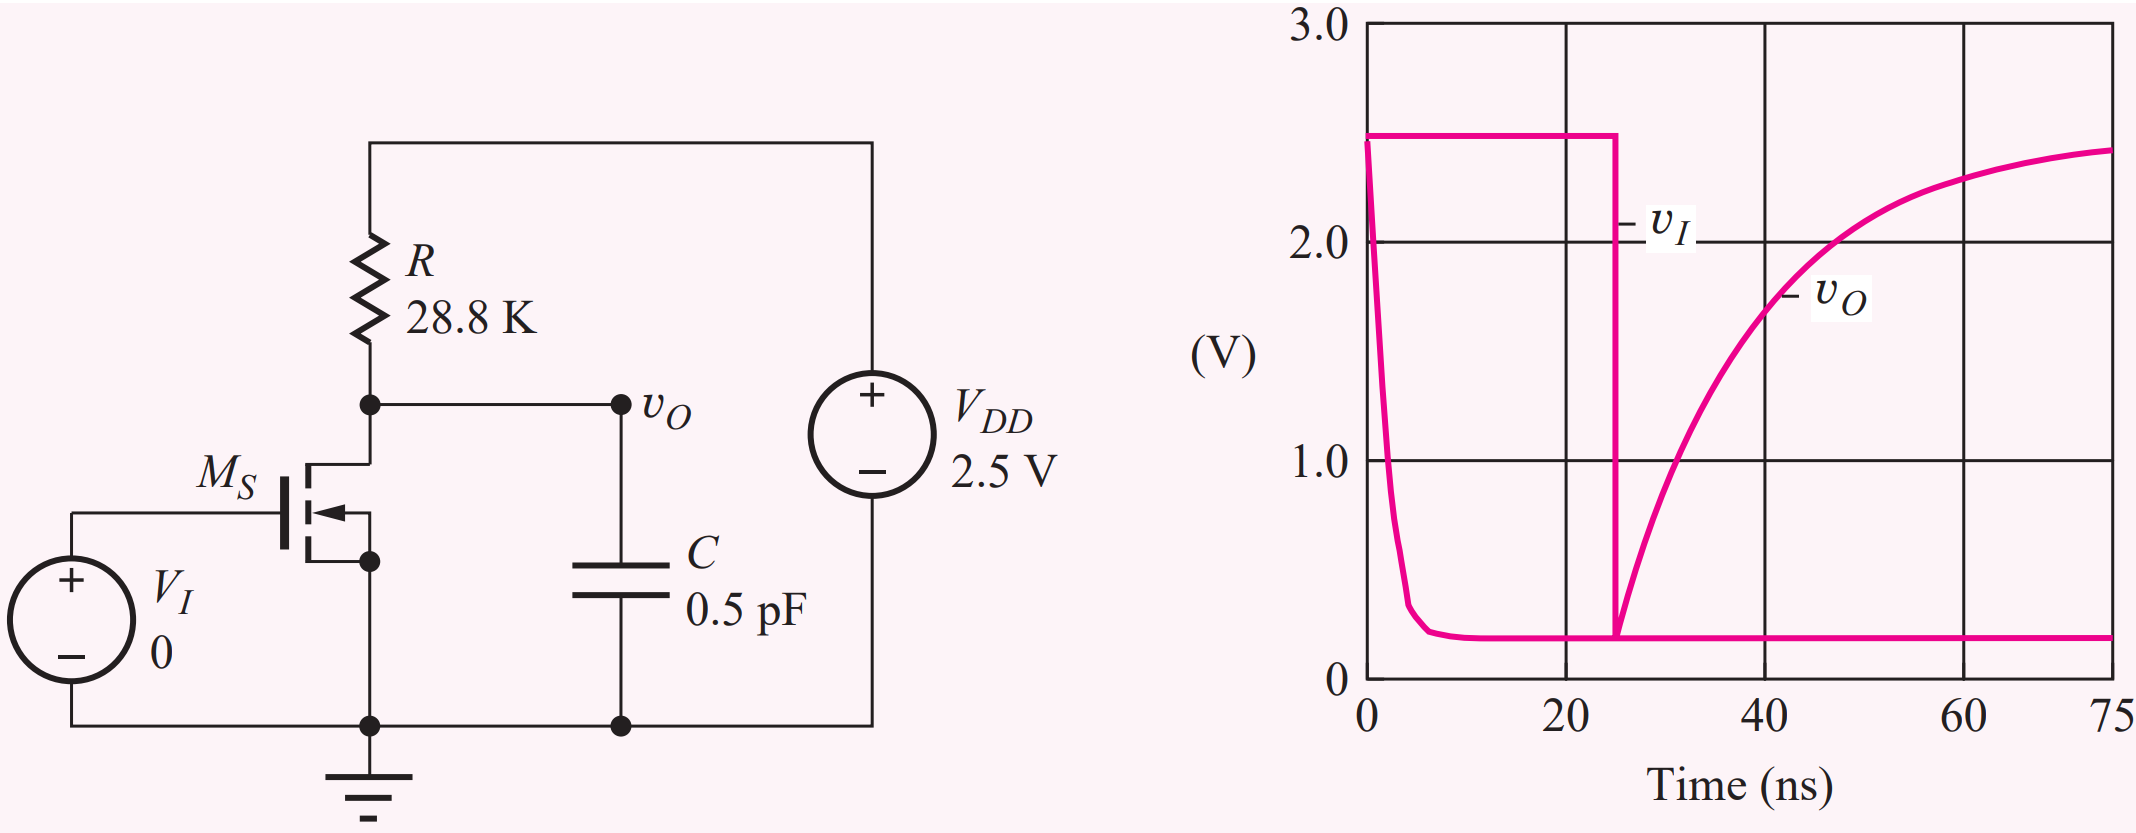
\includegraphics[width=0.5\linewidth]{img/spice.png}
    \caption{Simulazione Spice}    
\end{figure}
Il gradino raffigura l'ingresso, le curve rappresentano l'uscita.


\newpage
\subsection{Transitorio, invertitore pseudo nMOS}

Situazione	simile	alla	precedente,	approssimiamo	anche	 la	resistenza	del	pMOS di	carico

\begin{equation*}
    R_p = \frac{1}{K_p(\vdd - V_{TP})}\qquad\qquad K-p = 1.11\cdot40\,\frac{\mu A}{V^2}
\end{equation*}

\begin{equation*}
    R_p = \frac{1}{44.4(2.5-0.6)} = 11.9\,K\Omega
\end{equation*}
\begin{equation*}
    t_r = 3.7\cdot11.9\cdot0.5 = 22\,ns
\end{equation*}
\begin{equation*}
    t_{PLH} = 1.2\cdot11.9\cdot0.5 = 7.14 \,ns
\end{equation*}

\begin{figure}[htbp]
    \centering
    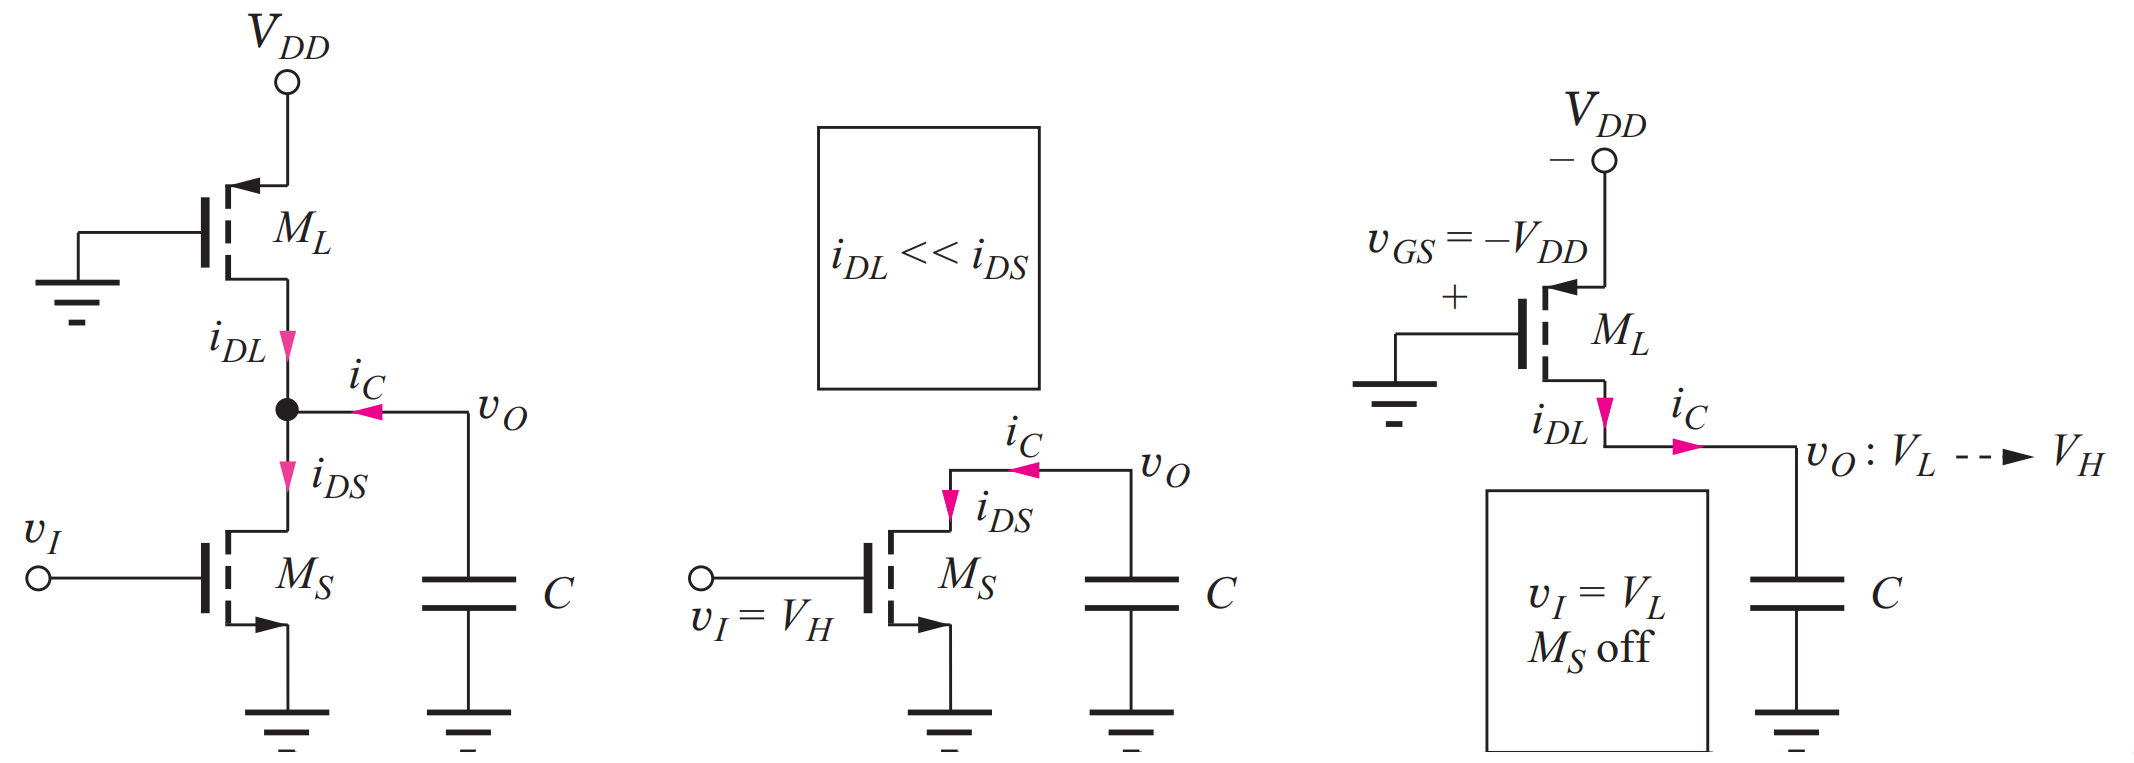
\includegraphics[width=0.85\linewidth]{img/transitorio_nMOS.png}
    \caption{Transistore nMOS}
    
\end{figure}


\subsection{Confronto di inverter}
I	diversi	inverter	nMOS hanno	lo	stesso	comportamento	
in	discesa, c’è	sempre	un	nMOS che	scarica	il	condensatore.

In	salita,	dipende	dal	pull	up, il	pMOS è	quello	con	la	maggiore	capacità	di	corrente,	ed	ha	
quindi	il	ritardo	minore.


\begin{figure}[htbp]
    \centering
    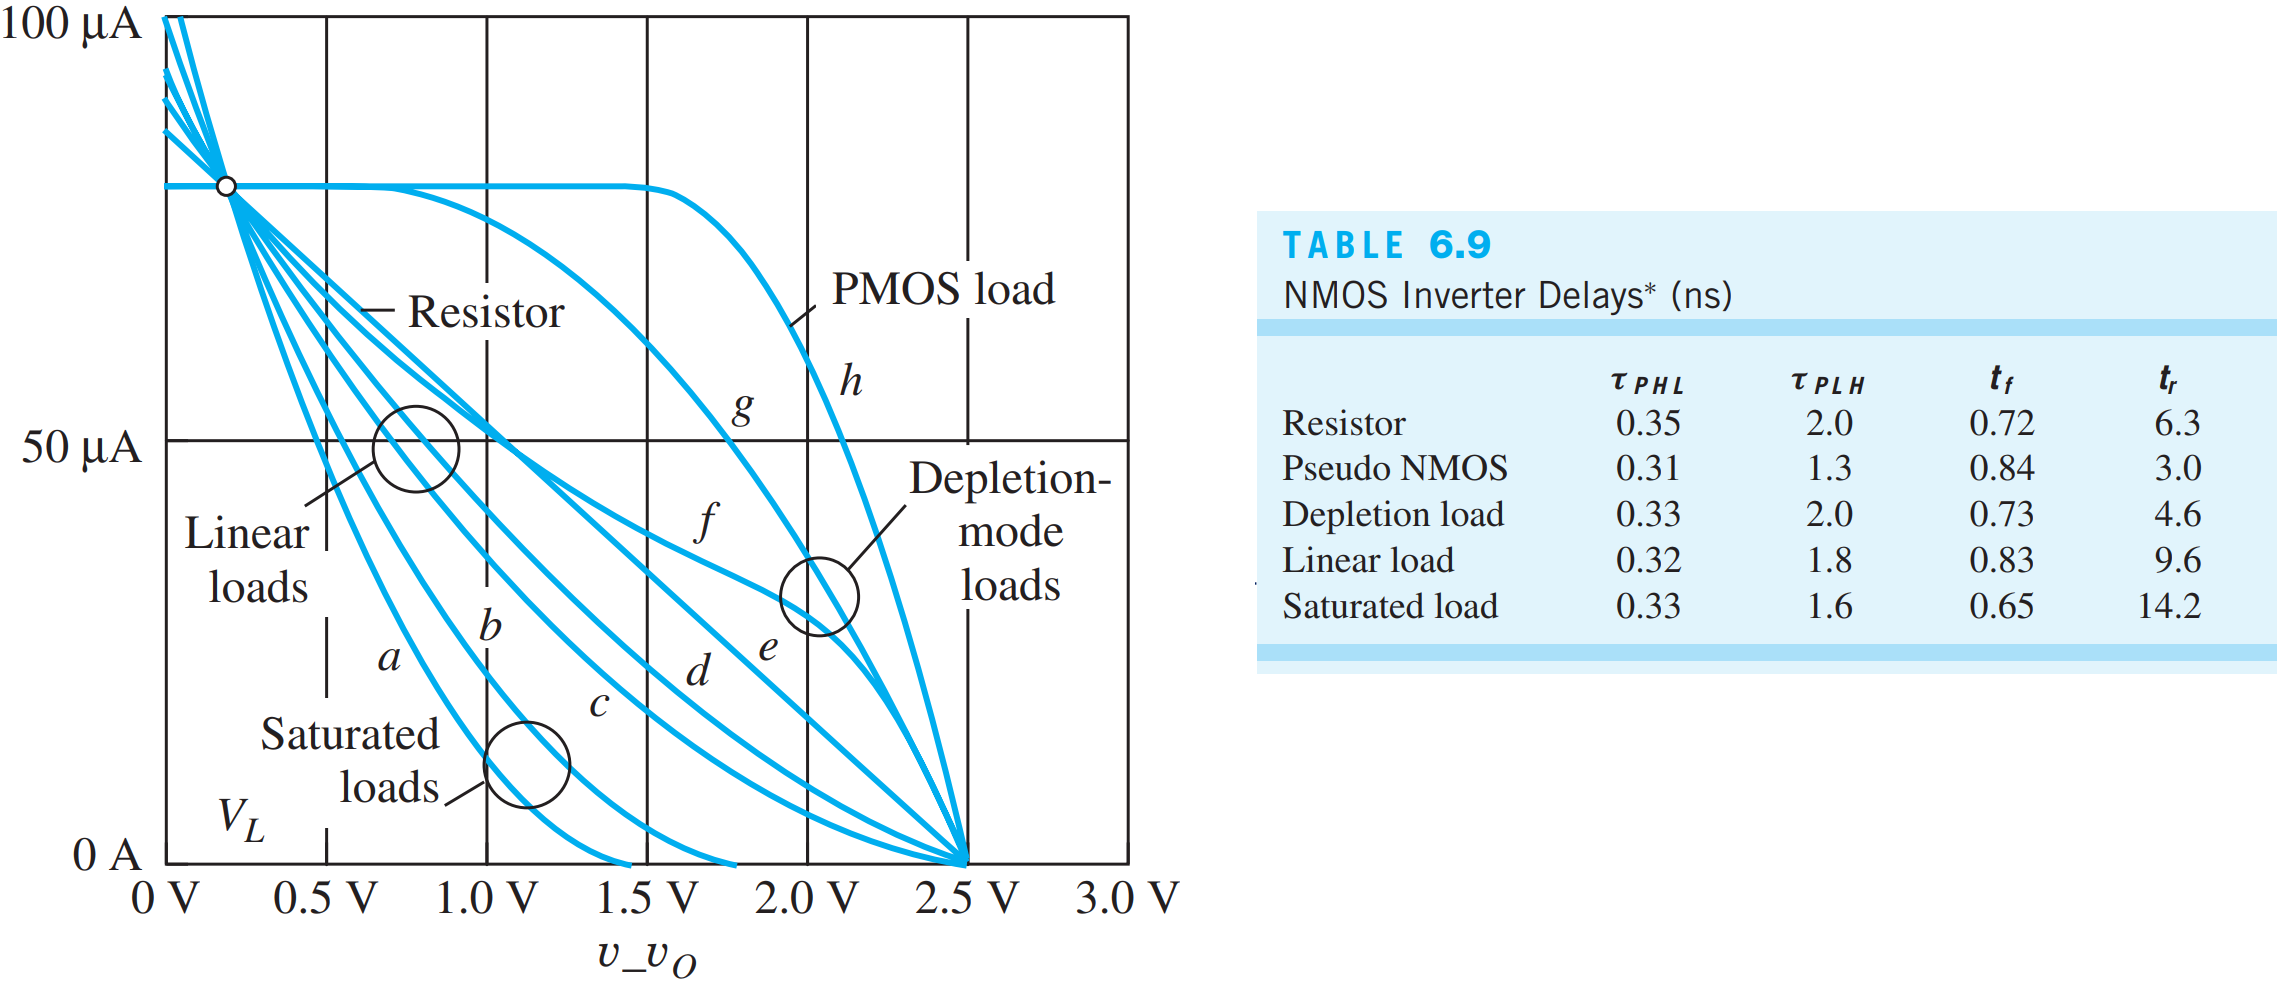
\includegraphics[width=0.75\linewidth]{img/cfr_inverter.png}
    \caption{Confronto dei vari inverter}    
\end{figure}

In tutti i casi trattati abbiamo considerato il cambiamento del ingressi istantaneo, ma quest'ultimo non avverrà istantaneamente e anche questo causa un ritardo.

\newpage
\section{Consumo	statico}

La porta logica consuma ogni qualvolta che passa corrente. Quando l'uscita è alta il pull-down è interdetto e il pull-up è attivo ma non consuma corrente (il gate a valle è carico, le cariche non devono passare), e infatti ai capi del resistore la differenza di potenziale risulta 0.

Consuma quando:

\begin{itemize}
    \item Deve passare dal valore zero al valore uno, passa corrente perché si deve caricare il condensatore
    \item Deve passare dal valore uno al valore zero, passa corrente perché deve passare corrente per scaricare il condensatore, in realtà stiamo dissipando la corrente caricata in precedenza.
\end{itemize}

Nel caso della logia a rapporto però, la porta consuma anche quando l'uscita è bassa e sta ferma, non consuma quando sta alta e ferma, perché il pull-down conduce, il pull-up pure e vi è una corrente che passa da $V_{DD}$ fino a massa. 

Questo consumo è definito \textbf{consumo statico} della porta logica.

\paragraph{Di quanta potenza si parla?}

\begin{equation*}
    P = V_{DD}I_{DD} = 2.5 \cdot80 = 200\,\mu W = 0.2\,mW \text{\,\,per non fare nulla!}
\end{equation*}

Il consumo medio si suppone essere la metà, $0.1\,mW$, dato la casualità dei due stati. 

\paragraph{Esempio:} con $10\,000$ porte logiche si ha un consumo statico di $1\,W$, oltre al consumo dinamico per far cambiare lo stato alla porta.

Si potrebbe diminuire la corrente statica aumentando la resistenza, ma andremo a peggiorare le prestazioni: aumenterà la costante di tempo per caricare il gate della porta logica.

Questo tipo di logica rimane un grande problema per sistemi complessi, non possiamo fare grossi circuiti perché costruiremo delle grandi stufe elettriche.

\paragraph{}
Queste porte non sono più usate, le abbiamo studiate per il concetto di base le quali ci introducono il \textbf{metodo di analisi} del pull-down, infatti ora analizzeremo il pull-up.

